\chapter{Evaluating the Feasibility of Monitoring Lipid Turnover using Heavy Water Loading and $^2$H Magnetic Resonance}
\label{Chap:Lipid}

\section{Introduction}

Adipose tissue (more commonly known as body fat) is key for energy storage and can be found either under the skin (subcutaneous fat) or around internal organs (visceral fat) as well as in bone marrow, in breast tissue and around muscles. The cells that make up this tissue are known as adipocytes which store energy as \ac{TG}, and the breakdown/turnover of adipocytes and \ac{TG} is thought to be a good indicator of metabolic health and homeostasis. Adipose tissue growth through enlargement of existing adipocytes (hypertrophy) is possible as well as by increases in pre-adipocyte and adipocyte numbers (hyperplasia), adipocyte death is also a vital part of the \ac{TG} turnover \cite{White2019DynamicsDisease}. The differences between these formations in adipose tissue informs vital information on cardiometabolic health \cite{Carnethon2002Serum19871998}. It was originally thought that adipocyte count increase only occurs during childhood and adolescence \cite{Salans1973StudiesPatients}, and that changes in weight are due to adipocyte size changes. However, new studies now show this is not the case \cite{White2016DifferencesWomen} which shows the importance of \textit{in vivo} studies into adipose tissue turnover.

\textit{In vitro} methods using cell cultures can be used to assess adipose/lipid turnover and can provide information about specific adipocyte growth and death \cite{Tchkonia2002FatPreadipocytes}. However, results from cell culture experiments do not necessarily provide insight into the turnover of lipids in tissue in the human body. One of the reasons for using \textit{in vitro} methodology is that the half-life of \ac{TG} \textit{in vivo} in humanshas been found to be $\sim$six months \cite{Strawford2004AdiposeO}, which can make it difficult to measure. However, lipid turnover can be measured by using $^2$H labelling through \ac{D$_2$O} ingestion and invasive tissue sampling (biopsy), with the analysis being performed using mass spectrometry and application of \ac{MIDA} \cite{White2019DynamicsDisease, Strawford2004AdiposeO, Belew2022DeTracers, Turner2003MeasurementMIDA}. Following heavy water loading, $^2$H makes its way into the glycerol moiety and fatty acid chains of triglycerides during lipid formation (lipogenesis) making it possible to measure TG synthesis \cite{Turner2003MeasurementMIDA}. Using this method differences in the \ac{TG} synthesis rate between healthy and insulin-resistant individuals \cite{Allister2015InHumans} and between different races \cite{White2018RacialHumans} have been evaluated. However, the need for biopsy restricts the range of tissue sites that can be sampled (e.g., making it difficult to sample visceral fat) and causes patient discomfort. Heavy water loading has previously been utilized in conjunction with magnetic resonance imaging and spectroscopy (\ac{MRI}/\ac{MRS}) allowing measurement of enhanced $^2$H MR signals fromwater and fat \textit{in vivo} \cite{Brereton1989TheMice, Cocking2023DeuteriumDosing}. The enrichment of $^2$H into \ac{HDO} that can be measured using \ac{MRI} or \ac{MRS} has been shown to follow physiological estimates and can therefore be accurately predicted \cite{Cocking2023DeuteriumDosing}, the enrichment into lipids is much slower \cite{White2019DynamicsDisease, Strawford2004AdiposeO} but can also be predicted \cite{White2019DynamicsDisease}.

\section{Theory}
\label{Chap:Lip:Theory}

The $^2$H MR signal that arises from naturally occurring \ac{HDO} \textit{in vivo} is $\approx$0.015\% (NA). Some of the $^2$H signal is lost ($L$)through urinating, breathing and sweating and is replenished through what we eat and drink, assuming the food and drink only contains naturally occurring $^2$H. As has already been shown it is possible to increase the \textit{in vivo} $^2$H abundance by ingesting extra $^2$H in the form of heavy water (or an aqueous solution of heavy water), in this case the volume of $^2$H lost will increase but it will not be enough to overcome the increase in consumption of $^2$H. The new $^2$H abundance in a day ($A_{t+1}$ as a percentage) can then be estimated on an iterative process, and is relative to a participants total body water (BW) which can be shown in Eq. \ref{eqn:Lip:HDO}.

\begin{equation}
    A_{t+1} = A_t + \frac{L[\textrm{NA} - A_t]}{\textrm{BW}} + \frac{D}{\textrm{BW}}
    \label{eqn:Lip:HDO}
\end{equation}

\noindent Where the original abundance is given as $A_t$, and the extra $^2$H consumed is given as $D$. This equation is useful when the extra $^2$H is ingested on a daily basis, the change in $^2$H abundance with respect to time ($dA/dt$) can then be calculated as a differential equation according to Eq. \ref{eqn:Lip:HDO_diff}.

\begin{equation}
    \frac{dA}{dt} = \frac{L[\textrm{NA} - A]}{\textrm{BW}} + \frac{D}{\textrm{BW}}
    \label{eqn:Lip:HDO_diff}
\end{equation}

\noindent It is noted that $L/$BW is the relative loss in water which would now be considered a constant rate ($\lambda_w$) along with the extra $^2$H consumed ($D$). An estimate for the relative loss $lambda_w\sim 3/41$ assuming 3 L of fluid lost and a BW of 41 L. It can be beneficial to look at the change in $^2$H abundance as a multiplicative change compared to NA ($E$). The differential equation then becomes Eq. \ref{eqn:Lip:HDO_diffE}.

\begin{equation}
    \frac{dE}{dt} = \lambda_w(1-E) + \frac{D}{\textrm{BW} \cdot \textrm{NA}}
    \label{eqn:Lip:HDO_diffE}
\end{equation}

\noindent Once loading ends ($D=0$) Eq. \ref{eqn:Lip:HDO_diffE} can be solved to give Eq. \ref{eqn:Lip:E}. Here the enrichment $E$ exponentially decays from $E_0$, the enrichment at the end of loading, to natural abundance ($E=1$). With a time constant $\lambda_w$.

\begin{equation}
    E = E_0 - \exp(\lambda_wt)
    \label{eqn:Lip:E}
\end{equation}

\noindent obviously to accurately calculate the enhancement of $^2$H in water accurate estimates for $L$ and BW are needed. It is difficult to accurately determine $L$ as it depends on an individual's lifestyle, however BW can be calculated. Line of best fits have been found that relate total body-water to anthropometric measurements (height ($H$), weight ($W$), age ($A$) and gender) \cite{Watson1980TotalMeasurements}, equations for the relationships are found in \ref{eqn:Lip:male} for males and Eq. \ref{eqn:Lip:female} for females.

\begin{equation}
    \textrm{BW(litres)} = 2.447-0.09516A\textrm{(years)}+0.1074H\textrm{(cm)}+0.3362W\textrm({kg})
    \label{eqn:Lip:male}
\end{equation}
\begin{equation}
    \textrm{BW(litres)} = -2.097+0.1069H\textrm{(cm)}+0.2466W\textrm({kg})
    \label{eqn:Lip:female}
\end{equation}

The change in lipid turnover is more complicated to analytically examine, and is often investigated. Data from lipid turnover studies looking at $^{14}$C content of fat show that the rate of lipid storage is $\sim$16 kg/year (44g/day) \cite{Arner2011DynamicsDisease, Spalding2017ImpactTissue}, which gives a time constant ($t_f$) for lipid turnover of $\sim$397 days. This estimate assumes a healthy 70 kg individual with a body fat of 25\%, with the value likely to vary dependent on the individual's size, \ac{BMI} and age. Using this value we can estimate the concentration of $^2$H in fat during and after a period of heavy water loading. The enhancement of the $^2$H concentration in fat from natural abundance depends on the decay rate ($\lambda_f = 1/t_f$) the number of days loaded ($t$), the water enhancement ($E$) and the fraction ($f$) of H atoms in CH$_2$/CH$_3$ groups. It has been found that $\sim$20\% of stored lipids arise from \ac{DNL}, which are more likely to derive from water, compared to triglycerides recycled from fatty acid breakdown. Of those stored lipids 1/3 of the H atoms come from water, and 2/3 come from the metabolite NADPH \cite{Zhang2017ChemicalNADPH}, conservatively the fraction ($f$) can therefore be approximated to a conservative 5\%. It is important to note that the H in NADPH can undergo catalytic exchange with water which can boost enhancement. If the water enhancement is approximated at x100 for 28 days, and assuming a range of $f$ of 5-20\% this gives an enhancement of 35-140\%. This enhancement should therefore theoretically be detectable using $^2$H MRS \textit{in vivo} \cite{Brereton1986PreliminarySpectroscopy}. 

As someone drinks heavy water, they can experience periods of dizziness and nausea \cite{Money1974HeavyAlcohol}, to mitigate this issue, the volume of heavy water drunk can be varied during the loading period \cite{Strawford2004AdiposeO, Cocking2023DeuteriumDosing}. To accurately calculate the estimated enhancement of $^2$H in lipids the lipid turnover and varying heavy water volume to be accounted for. This can be done by iteratively and numerically solving the differential Eq. \ref{eqn:Lip:Diff}.

\begin{equation}
    \frac{dS}{dt} = \lambda_f(f(E-1)+1-S)
    \label{eqn:Lip:Diff}
\end{equation}

\noindent where $S$ is the signal enhancement of $^2$H in lipids, and as before $E$ is the enhancement of the $^2$H in water. Example loading regimes, \ac{HDO} enhancements and corresponding signal enhancements in lipids according to Eq. \ref{eqn:Lip:Diff} are shown in Fig. \ref{eqn:Lip:Diff}. This solution has a similar form to the analytical expression in Eq. \ref{eqn:Lip:Load} (during loading).

\begin{equation}
    S = 1 + f(E_0 - 1)(1 - \exp(-\lambda_ft)
    \label{eqn:Lip:Load}
\end{equation}

 the cessation of loading that changes the analytical form of $E$ in Eq. \ref{eqn:Lip:E} needs to be accounted for in $S$. This is done in Eq. \ref{eqn:Lip:Full} by introducing the time constant $\lambda_w$, where $S_0$ is the enhancement in fat achieved at the end of the loading period.

\begin{equation}
    S = (S_0 - 1)\exp(-\lambda_ft)+\frac{\lambda_f}{(\lambda_w - \lambda_f)}f(E_0 - 1)[\exp(-\lambda_ft)-\exp(-\lambda_wt)]
    \label{eqn:Lip:Full}
\end{equation}

 Either Eq. \ref{eqn:Lip:Diff} or Eqs. \ref{eqn:Lip:Load} and \ref{eqn:Lip:Full} are used to predict the amount of lipids that should be detectable using $^2$H \ac{MRI}/\ac{MRS}. Both prediction methods estimate an increase in fat signal of 30-40\%, this level of enhancement should be detectable and could therefore inform on metabolic health. 
 
 As a precursor to tracer studies we have explored the deuterium spectrum obtained from the lower leg at \ac{NA} in four healthy human participants, characterising the T$_1$ and T$_2^*$ relaxation times of the two spectral lines and demonstrating that measurements are feasible at 3T magnetic field strength on a clinical scanner using a transceive, surface \ac{RF} coil. We also evaluate whether $^2$H MR at 3T in conjunction with \ac{D$_2$O} loading could be used for non-invasive monitoring of lipid turnover in human subjects as an alternative to a methodology that uses \ac{D$_2$O} loading in conjunction with invasive biopsy. Three different healthy male participants were loaded for approximately four weeks and are scanned weekly or fortnightly for approximately sixteen weeks using $^2$H \ac{CSI} images.

\section{Methodology}

\subsection{\ac{NA} Scanning}

T$_1$ relaxation times of \textit{in vivo} \ac{HDO} and lipid signals in four different healthy human participants were measured at 3T in the Calf \cite{Damion2021NaturalT}. Scanning was performed on a 3T scanner (Philips Achieva) using an in-house built surface coil (5 cm diameter) tuned to the deuterium resonance 19.6 MHz. Which was placed under the calf muscle of the left leg. Non-localised \ac{IR} spectra were acquired at \ac{NA}, using a 900 Hz bandwidth adiabatic pulse followed by an inversion delay and then a non-selective \ac{RF} pulse of 90$^\circ$ nominal flip angle. Inversion times were $\tau$ = {5, 10, 20, 40, 80, 160, 320, 1000} ms, for a fixed \ac{TR} = 1200 ms (time between adiabatic pulses). \ac{FID}s were collected with 512 samples, NSA = 128, \ac{BW} = 3000 Hz. FIDs were truncated, zero-filled to 512 points, and line-broadened by 5 Hz exponential filter. % The pulse sequence used to obtain this data can be viewed in Fig. \ref{fig.pulse}. 

\begin{figure}
    \centering
    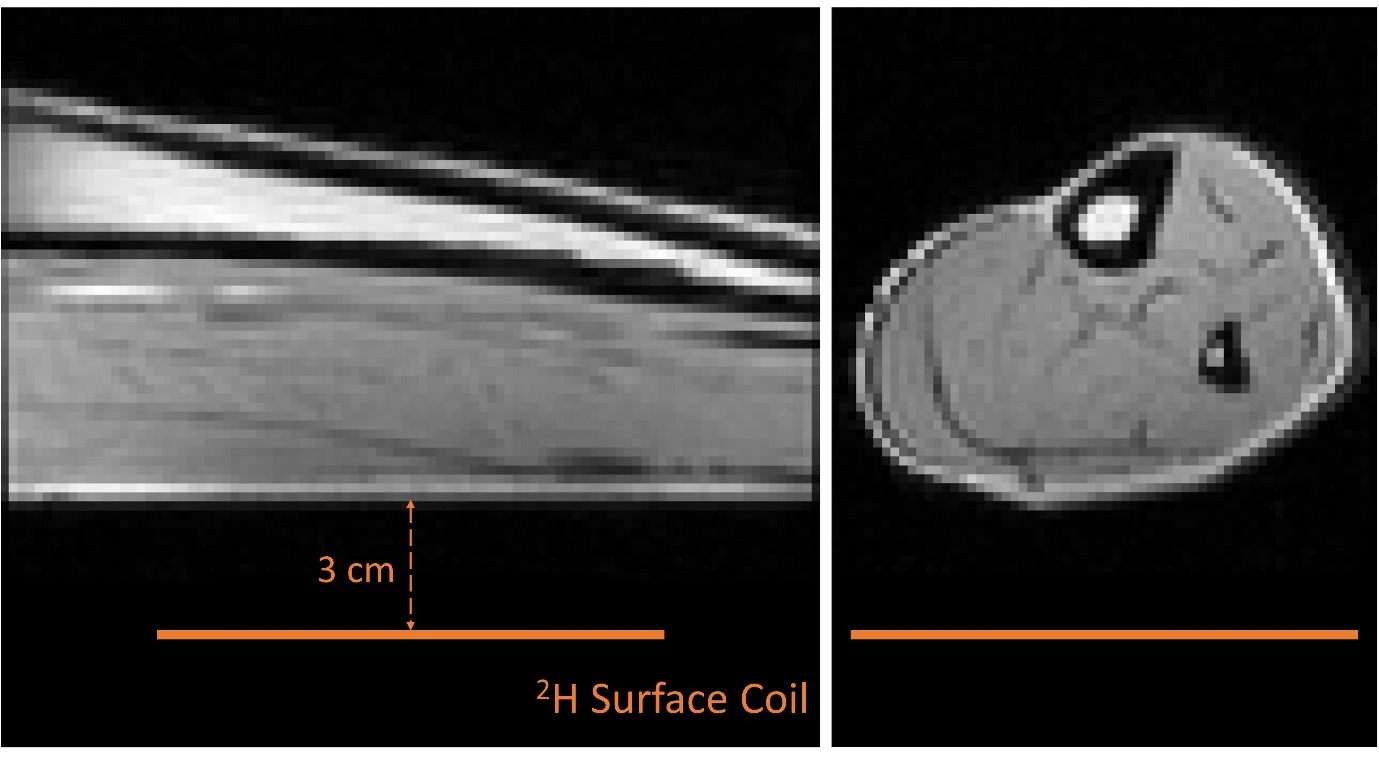
\includegraphics[width=1\textwidth]{Figures/Lipid/Coil.jpg}
    \caption{\textit{$^1$H images of the calf (FoV: 128 x 128 x 192 mm$^3$) also showing the position and extent of the $^2$H surface coil. Left image: mid-sagittal slice. Right image: mid-axial slice.}}
    \label{fig:Lip:Coil}
\end{figure}

The data was analysed using code written in MATLAB (MathWorks, Natick, USA). Spectra acquired with a surface coil over a large volume can possess peaks with different phases due to the averaging of various \ac{RF} factors over spatial distributions which are different for the molecules producing the spectral peaks. Therefore, a global zeroth-order phase-correction cannot be applied. Instead, the complex spectra were fitted to a sum of two complex Lorentzian lineshape functions employing independent phases for each spectral peak, as well as amplitude, frequency, and R$_2^*$. The inappropriateness of a simple phase-correction and the fact that the phases are functions of inversion time (other than the usual phase-shift at the null-point) mean that the inversion-recovery curve also needs to be analysed as a complex function:

\begin{equation}
    M(\tau) = \alpha - \beta\exp(-\frac{\tau}{T_1}) + (\beta - \alpha)\exp(-\frac{T_R}{T_1})
    \label{eqn:Lip:IR}
\end{equation}

where $M(\tau)$ is the complex magnetization (determined by the spectral amplitude and phase). The T$_2^*$ relaxation times for each peak were obtained from the fit of the Lorentzian and averaged over all inversion delays, the T$_1$ relaxation time was found from the fit of the \ac{IR} curve for each peak. Two peaks were consistently measured in all spectra. The chemical shift separation of these peaks was measured to be 3.55 $\pm$ 0.12 ppm. An example of the spectra that were acquired at different inversion times can be seen in Fig. \ref{fig:Lip:IR}.

\subsection{Fat Measurements by D$_2$O Loading}

The second study involved measuring $^2$H signals from the calf and abdomen in three different healthy male participants who underwent 28-days of drinking a mixture of heavy and regular water (D$_2$O/H$_2$O: 70/30\%). Fig. \ref{fig:Lip:Load} shows the loading schedules that participants followed, plus estimates of the expected changes in water and fat signals over 120 days. During loading the most \ac{D$_2$O} that was ingested at once was 150 ml, this slowing down of initial ramping of $^2$H enrichment meant that side effects of the loading were minimised compared to the protocol described in Chapter \ref{Chap:D2O}. No reports of dizziness or nausea were reported during initial loading. Using the equations described in Section \ref{Chap:Lip:Theory} we find that the $^2$H signal from water, increases to approximately 100x\ac{NA} in the loading period and then decreases after loading ceases, halving in amplitude every $\sim$6 days (Fig. \ref{fig:Lip:Load}). The fat signal rises more slowly to a maximum of 1.3-1.4 x\ac{NA} and then slowly decreases, as is also shown in Fig. \ref{fig:Lip:Load}.

\begin{figure}
    \centering
    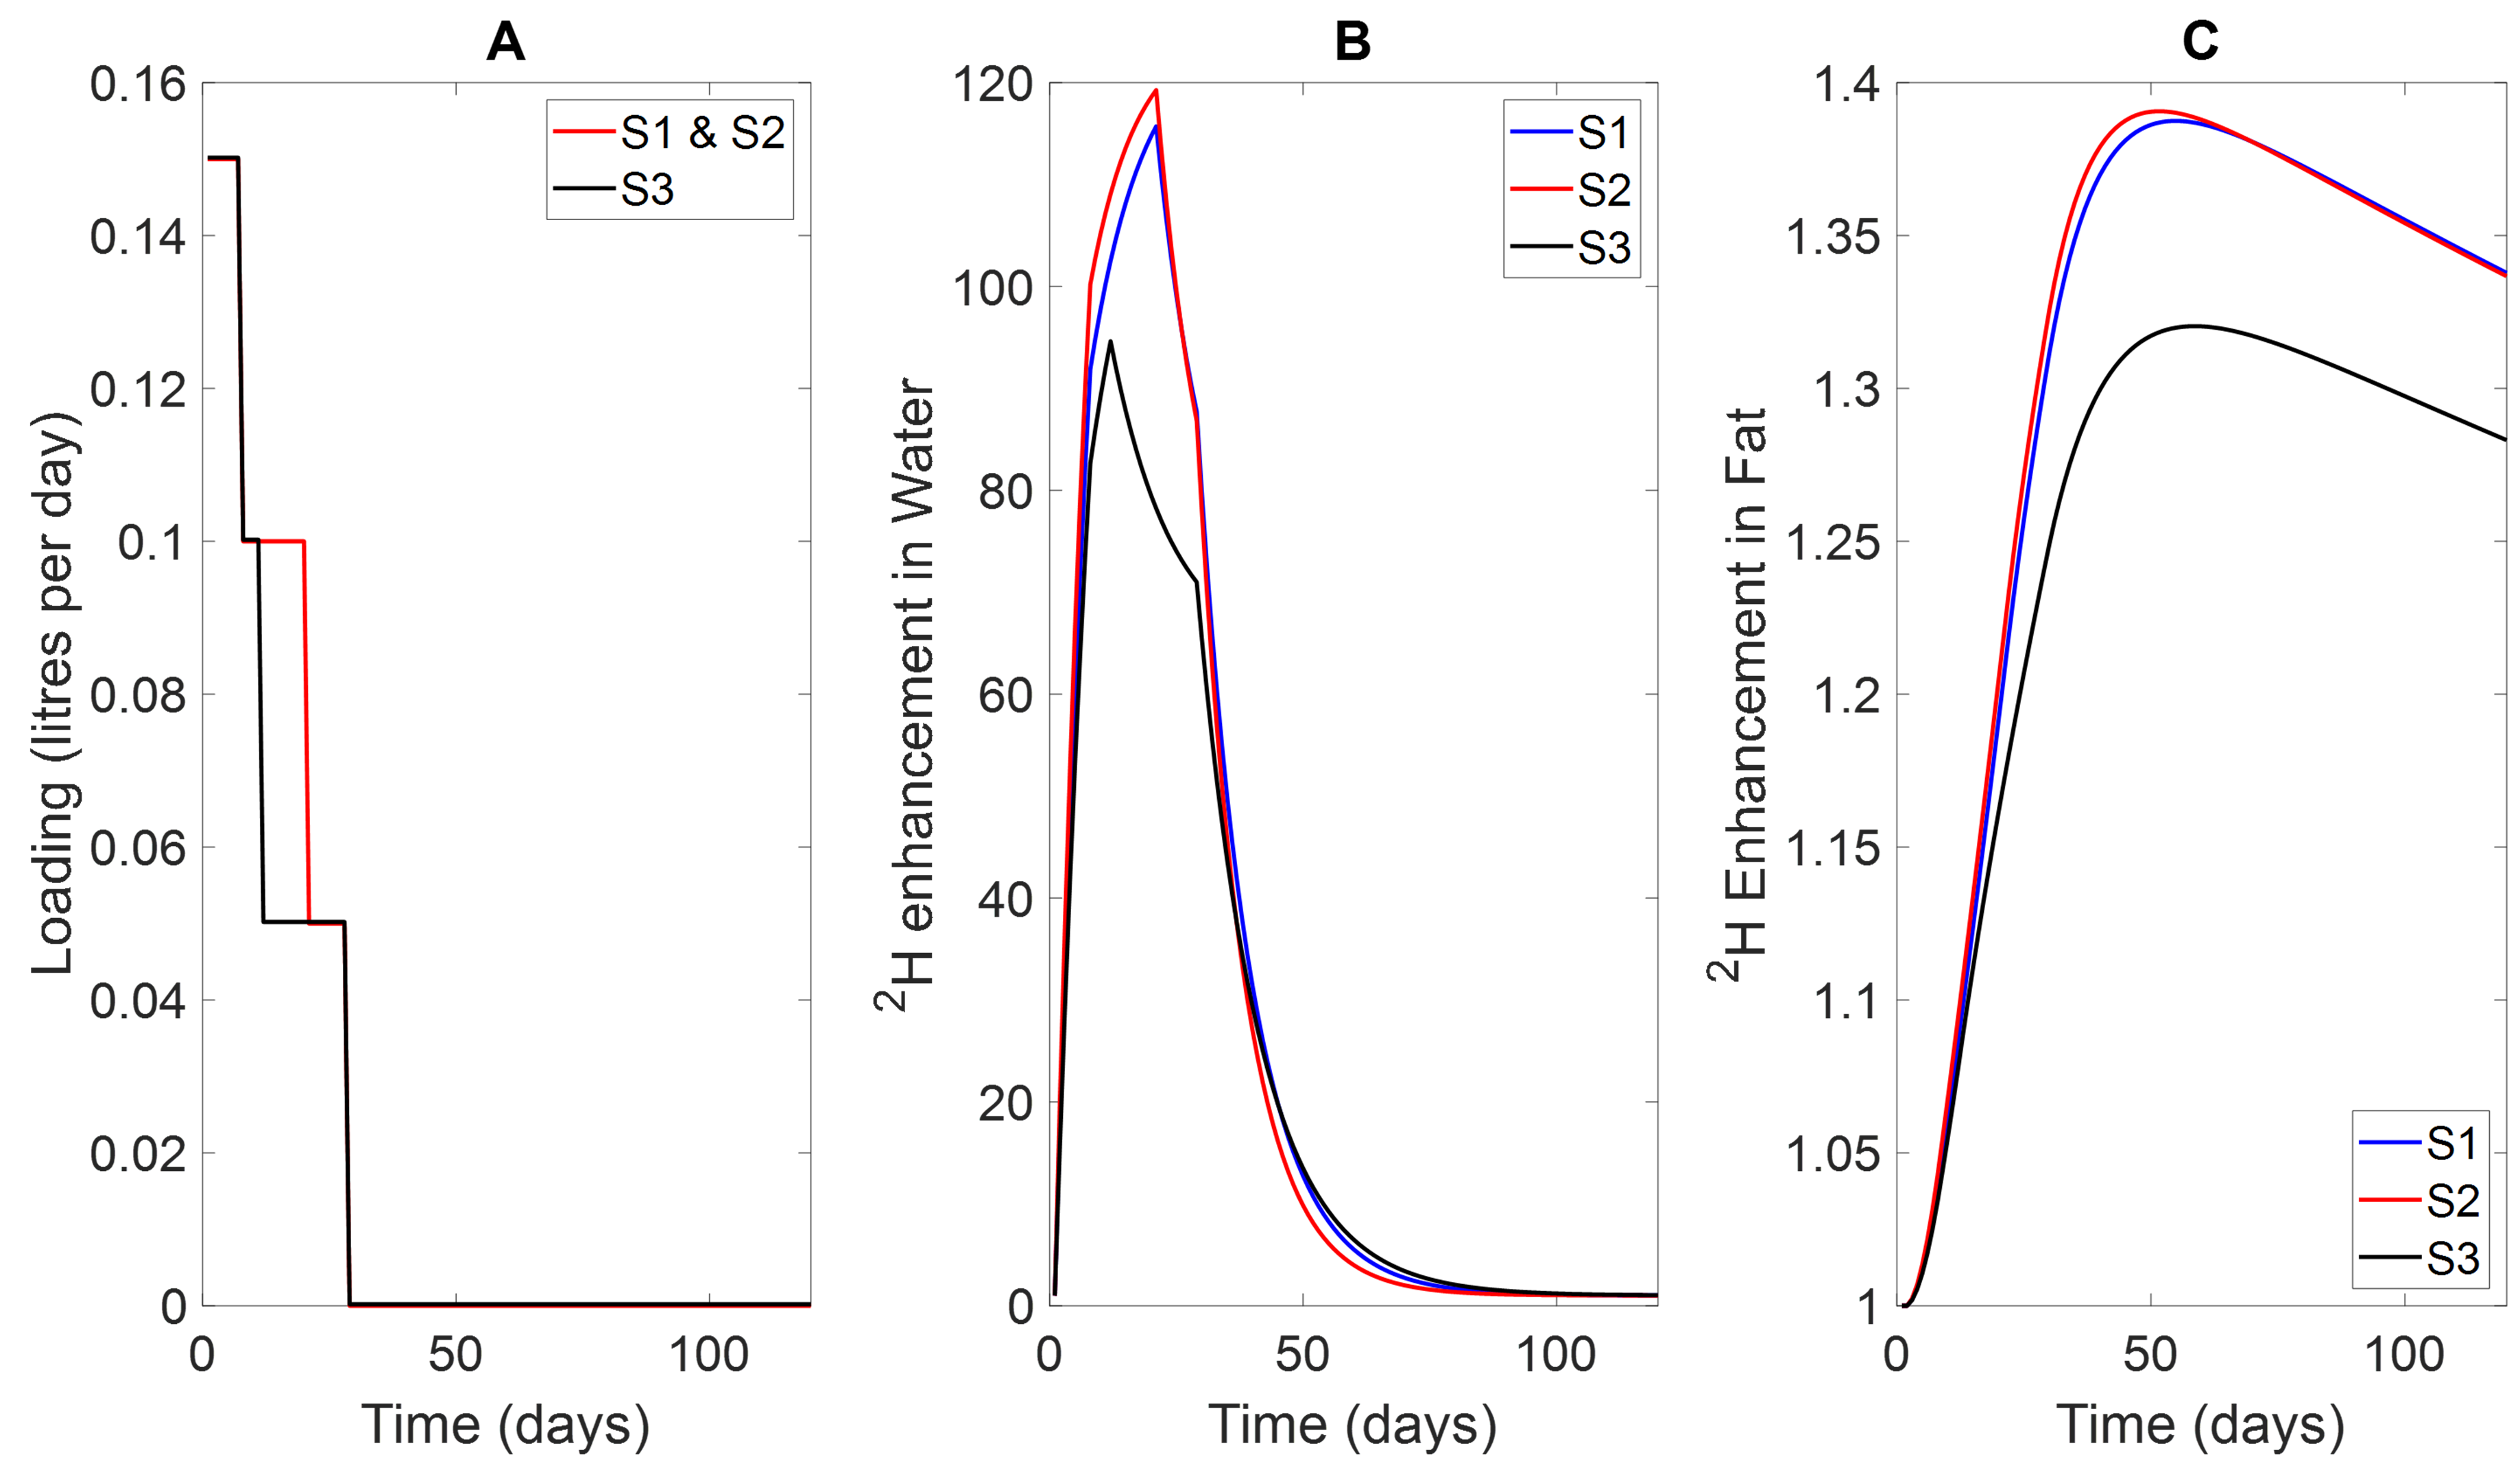
\includegraphics[width=1\textwidth]{Figures/Lipid/Loading_Routine.png}
    \caption{\textit{(A) Loading regimes followed by the three subjects: volume of 70\% D2O/30\% H$_2$O ingested per day. (B) Estimated signal enhancement in water signal relative to NA. (C) Estimated signal enhancement in fat relative to NA. These values were estimated using individual subject’s weight, height, and age, assuming 3.75 litre water turn-over per day, lipid half-life of 270 days \cite{Arner2011DynamicsDisease, Spalding2017ImpactTissue}; 5\% of hydrogen atoms in fatty acid chains of new lipids derived from water \cite{Turner2003MeasurementMIDA}.}}
    \label{fig:Lip:Load}
\end{figure}

Scans were performed on the same 3T scanner equipped with different in-house built $^2$H surface coils (5 cm-diameter for calf; 12 cm for abdomen, more detail can be found in Chapter \ref{Chap:Theory:Coils}). Measurements were made before loading, to characterise \ac{NA} signals, and then every $\approx$14 days during/after loading for a further 8 sessions. Anatomical landmarks were used to position the coils over the same region for each scan (under the calf/adjacent to the right abdomen near the liver). The calf/abdomen scanning sessions included a $^1$H scout scan; a $^1$H 3D gradient echo (\ac{GE}, \ac{FOV}: 128x128x192 / 446x446x250 mm$^3$, 2 mm isotropic voxels, \ac{TE} = 2.1/1.6 ms, TR = 20 ms, T$_\text{scan}$ = 122/88 s); bulk $^2$H spectra (\ac{FOV} = 300x300x12 mm$^3$, \ac{TR} = 50 ms, \ac{BW} = 2000 Hz, \ac{TE} = 0.37 ms, samples = 64, NSA = 256, T$_\text{scan}$ = 13 s); 1D $^2$H \ac{CSI} (\ac{FOV} = 300x300x150/300x300x140 mm$^3$, voxel size = 300x300x15/300x300x20 mm$^3$, \ac{TR} = 50 ms, \ac{BW} = 2000, \ac{TE} = 1.8/1.7 ms, samples = 64, NSA = 1024, T$_\text{scan}$ = 136/91 s) and 3D $^2$H \ac{CSI} (\ac{FOV} = 150x150x200 / 140x140x200 mm$^3$, voxel size = 15x15x20/20x20x20 mm$^3$, TR = 50 ms, \ac{BW} = 2000 Hz, \ac{TE} = 1.7 ms, samples = 64, NSA = 36/48, T$_\text{scan}$ = 520/420 s). Before loading started and at the end of the loading period, subjects were scanned multiple times with inter-scan repositioning to allow estimation of fractional signal variation due to positioning errors. A \ac{TR} of 50 or 70 ms was used to maximise the \ac{SNR} of the signal from fat. A full list of scan parameters can be found in Table \ref{fig:Lip:Scan_Detail}, it does not include details when a \ac{TR} of 70 ms was used.

\begin{table}
    \centering
    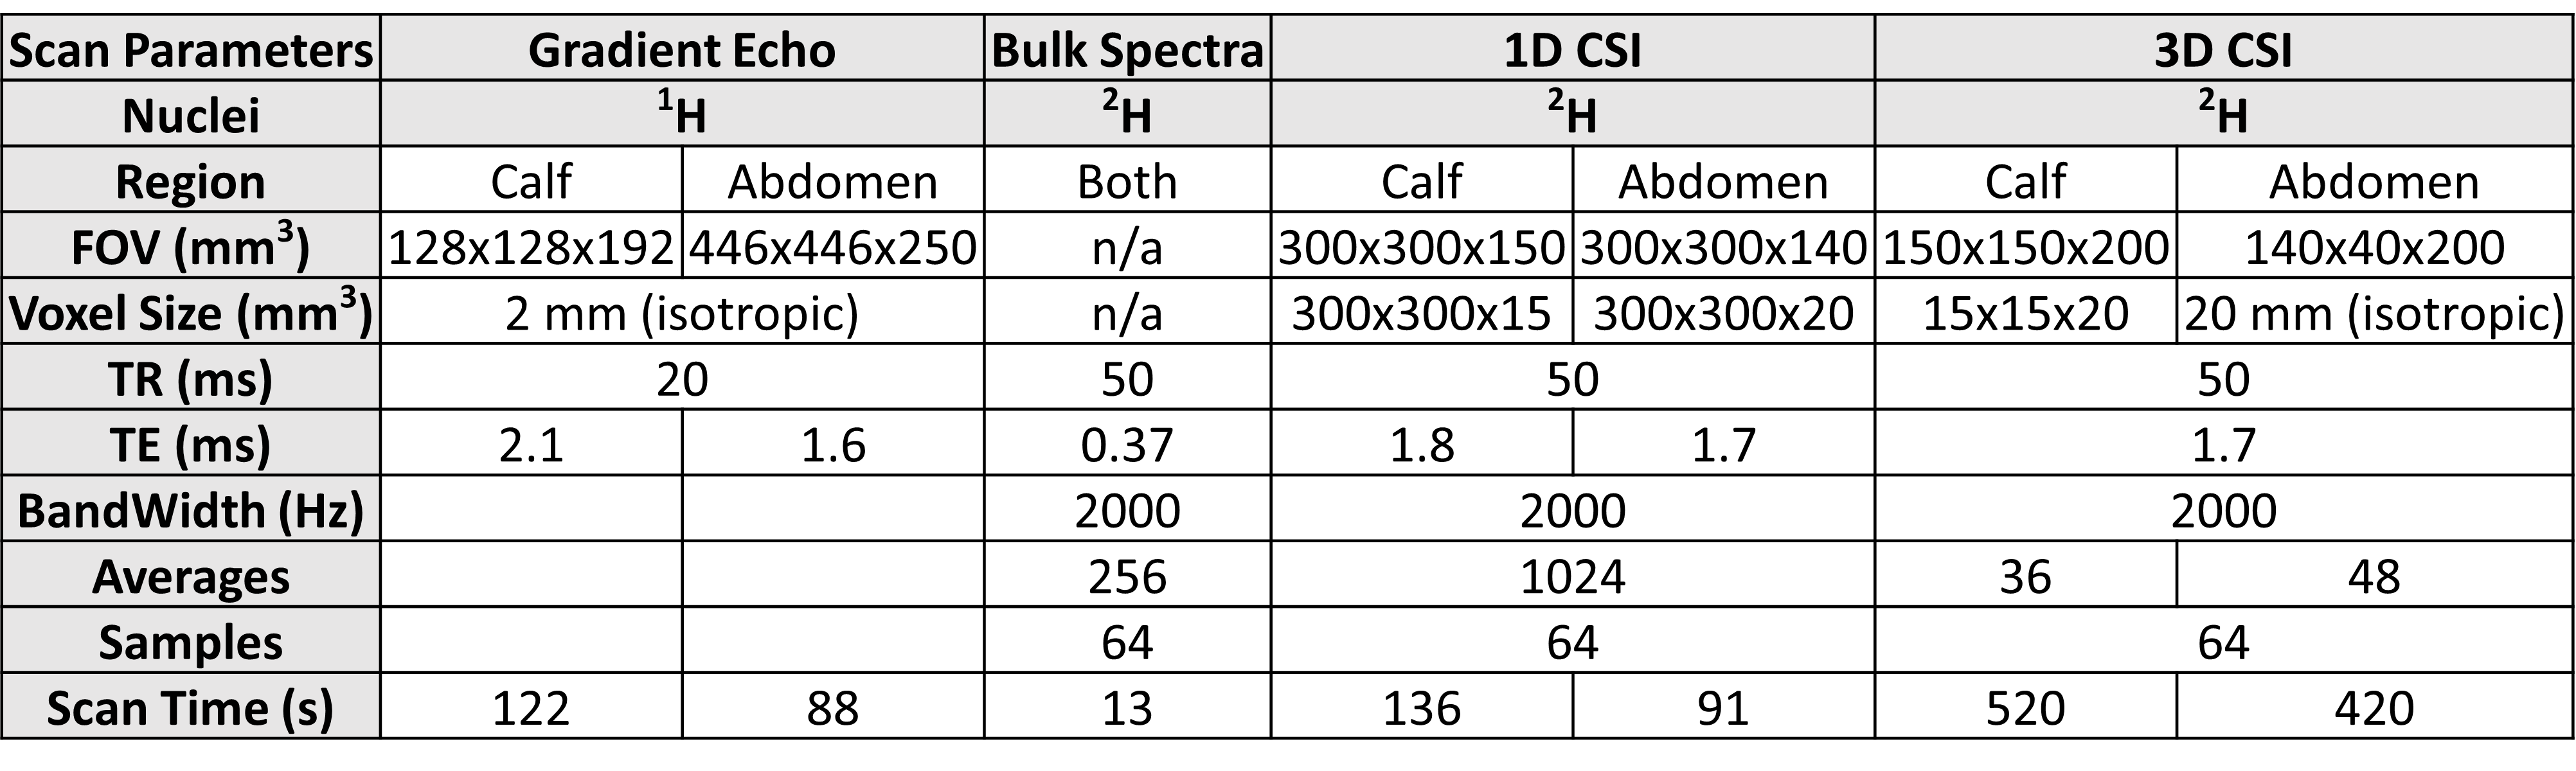
\includegraphics[width=1\textwidth]{Figures/Lipid/Scan_Details.png}
    \caption{\textit{The imaging and spectroscopic scan parameters used to investigate fat increases following D$_2$O loading for both regions (calf and abdomen). CSI measurements were also obtained with a \ac{TR} of 70 ms.}}
    \label{fig:Lip:Scan_Detail}
\end{table}

Code written in MATLAB (MathWorks, Natick, USA) using the OXSA-AMARES \cite{Purvis2017OXSA:MATLAB} toolbox was used to fit each voxel to a model incorporating water and fat peaks; in the calf, the water signal was modelled as a doublet with equal amplitudes (due to quadrupolar splitting) \cite{Gursan2022ResidualMuscle}. Water peaks were fit with a chemical shift $\approx$4.8 ppm with a lipid peak at $\approx$1.3 ppm, both sets peaks shared the same phase in fitting. To produce single measures of signal enhancement with reduced sensitivity to \ac{FOV}-positioning, we averaged fat and water signal amplitudes over \ac{ROI} (3x3x3/3x5x3 voxels for the calf/abdomen) sited relative to the voxel with maximum water signal (i.e., over the centre of the surface coil) to obtain a water value, and shifted 1 voxel closer to subcutaneous fat (right for abdomen, posterior for calf) to obtain a lipid value.

\section{Results}

\begin{figure}
    \centering
    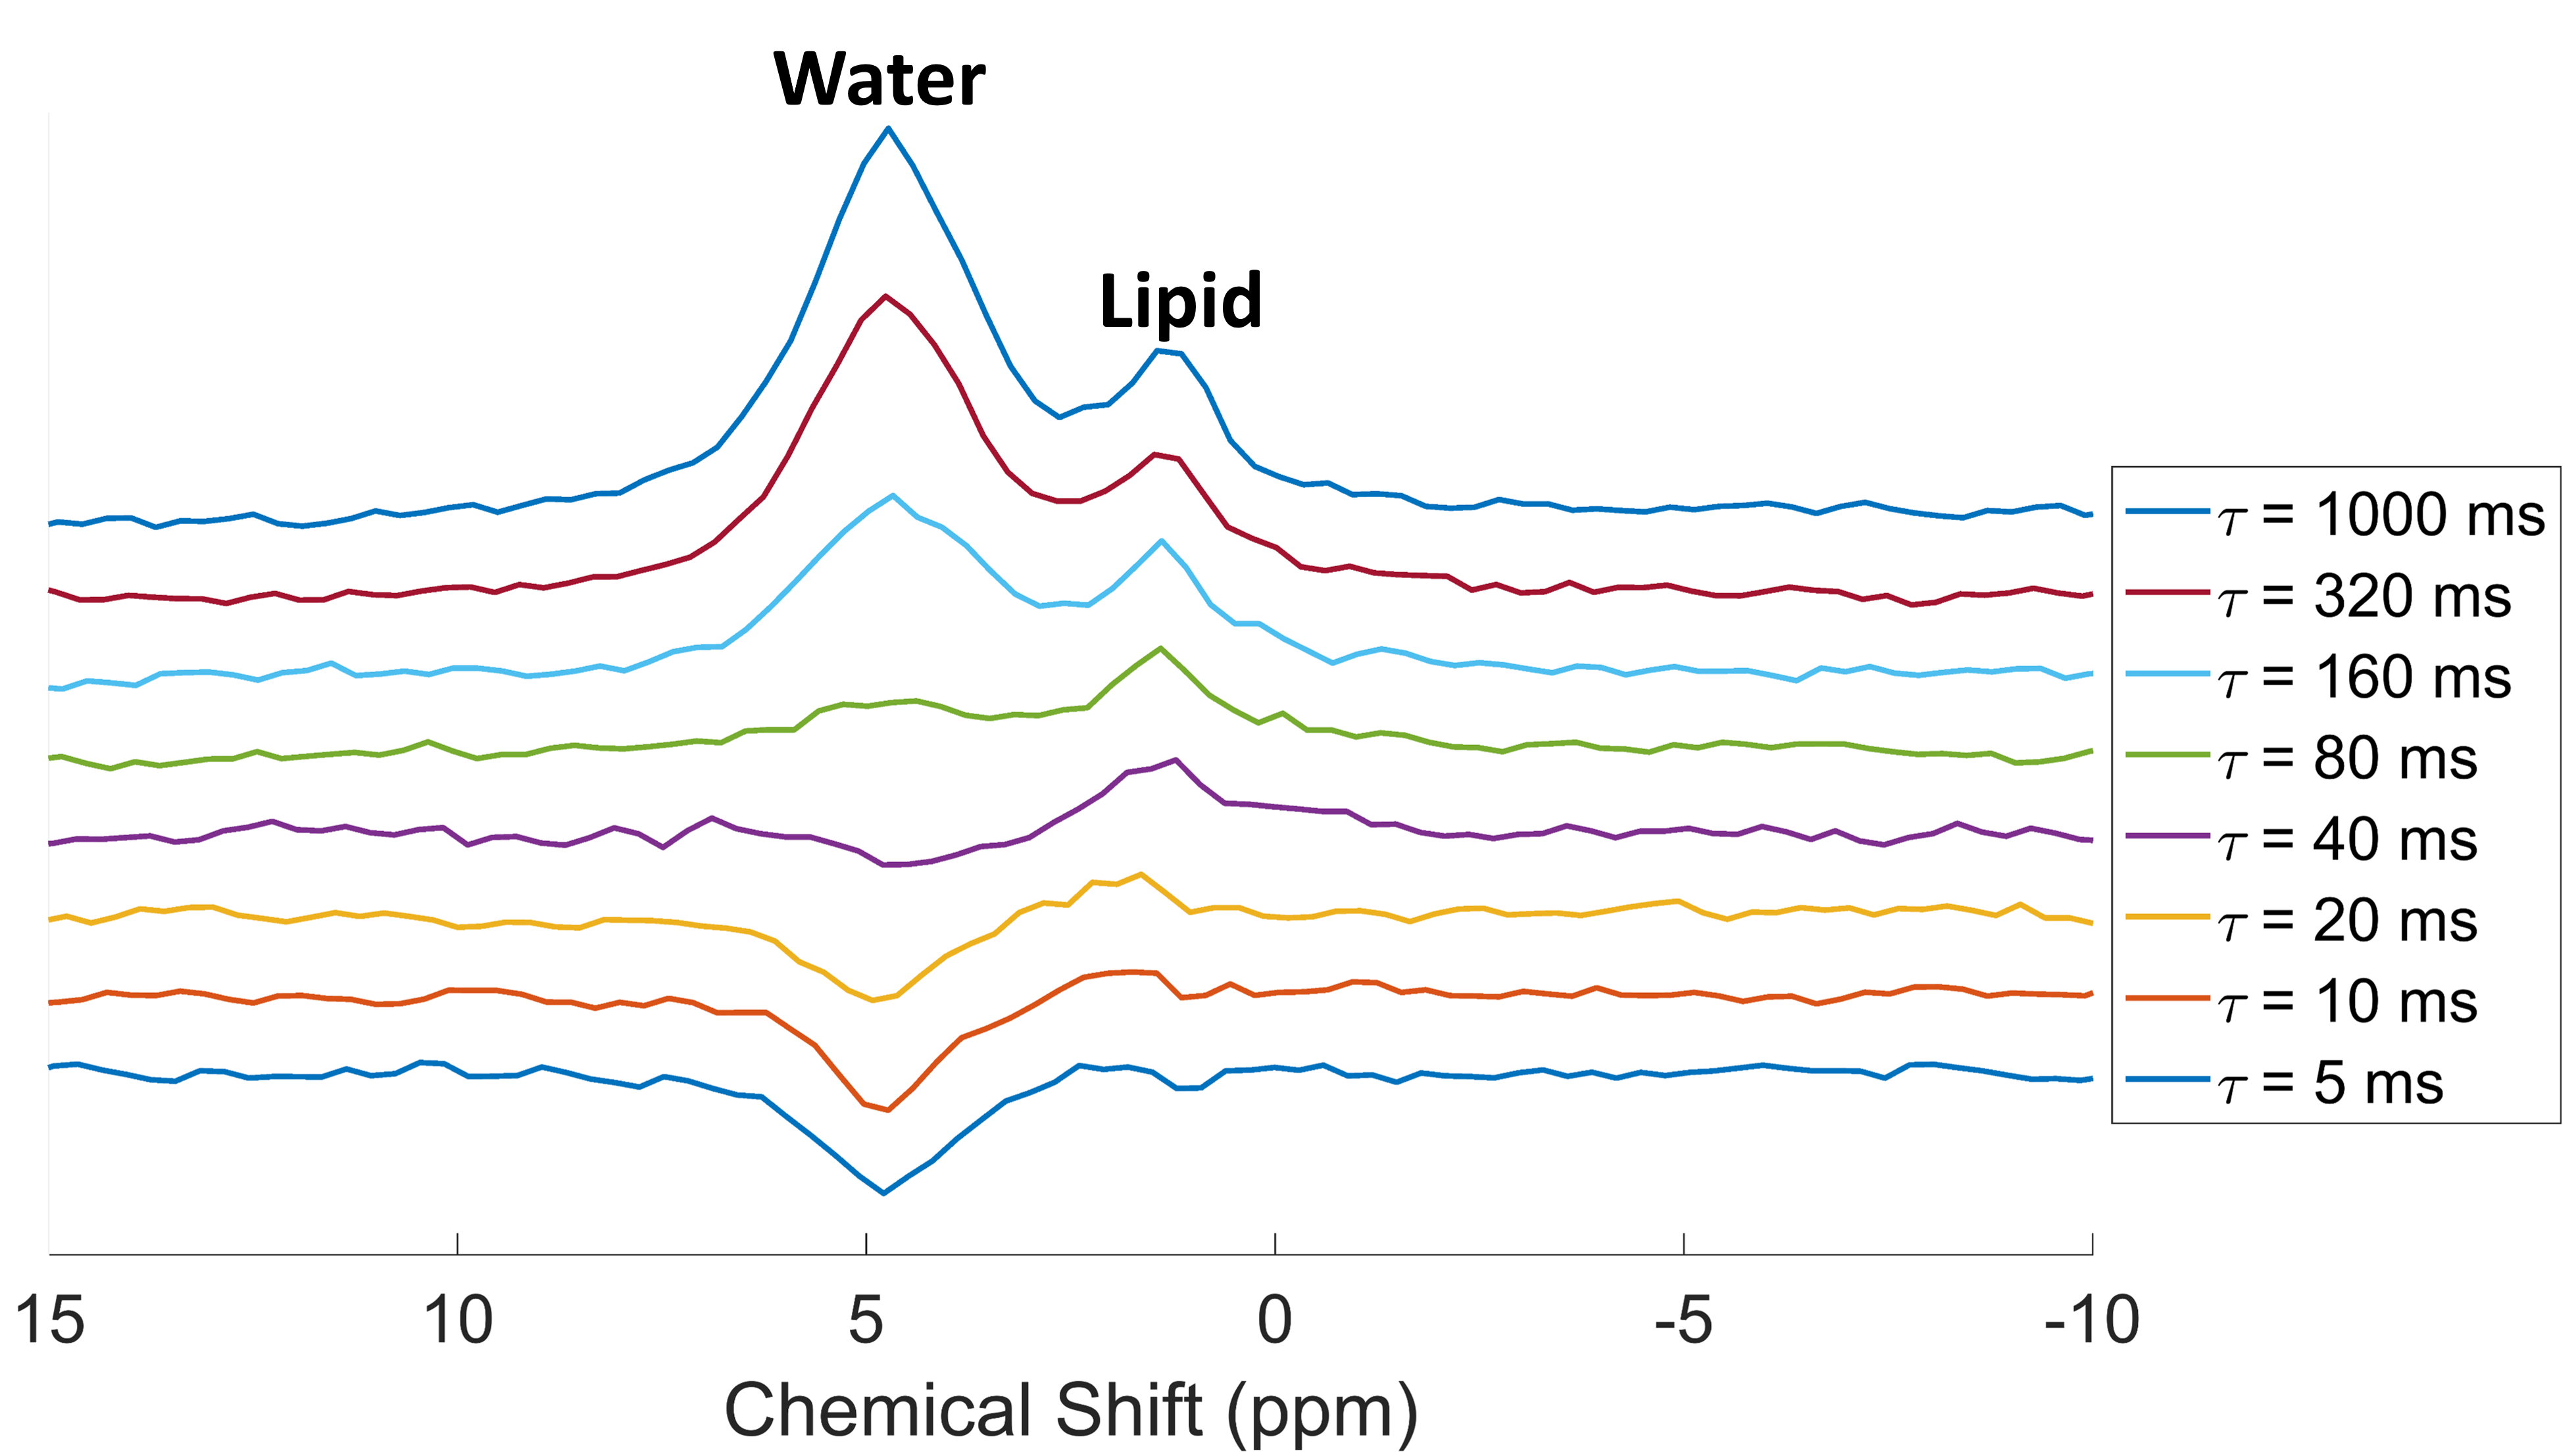
\includegraphics[width=1\textwidth]{Figures/Lipid/NA_IR.png}
    \caption{\textit{\textit{In vivo} spectra obtained during an inversion-recovery experiment. At varying inversion times ($\tau$) ranging from 5 to 1000 ms which are given in the legend, in milliseconds.}}
    \label{fig:Lip:IR}
\end{figure}

\subsection{Relaxation Time Values}

The largest peak in Fig. \ref{fig:Lip:IR} corresponds to the HDO present in the calf, whilst the second smaller peak is theorised to originate from CHD groups from adipose tissue (body fat). Two peaks are clearly visible: a water peak (\ac{HDO}) and a peak at 3.5 ppm lower. After correcting for applied line-broadening, mean T$_2^*$ values were obtained for \ac{HDO} of 8.2 $\pm$ 1.6 ms, and 14.0 $\pm$ 2.5 ms for lipids (n=4, see Table \ref{fig:Lip:R_Table}). Figure \ref{fig:Lip:IR} shows a set of spectra acquired during an \ac{IR} experiment. All spectra were globally shifted in reference to the spectrum of longest inversion time. Figure \ref{fig:Lip:Amp_Tau} shows the complex spectral amplitudes and their fitted lines according to Eq. \ref{eqn:Lip:IR}, for each of the two peaks (\ac{HDO} and lipids). Mean T$_1$ values were found to be 199 $\pm$ 34 ms for \ac{HDO} and 56 $\pm$ 10 ms for lipids (n=4, see Table \ref{fig:Lip:R_Table}).

\begin{figure}
    \centering
    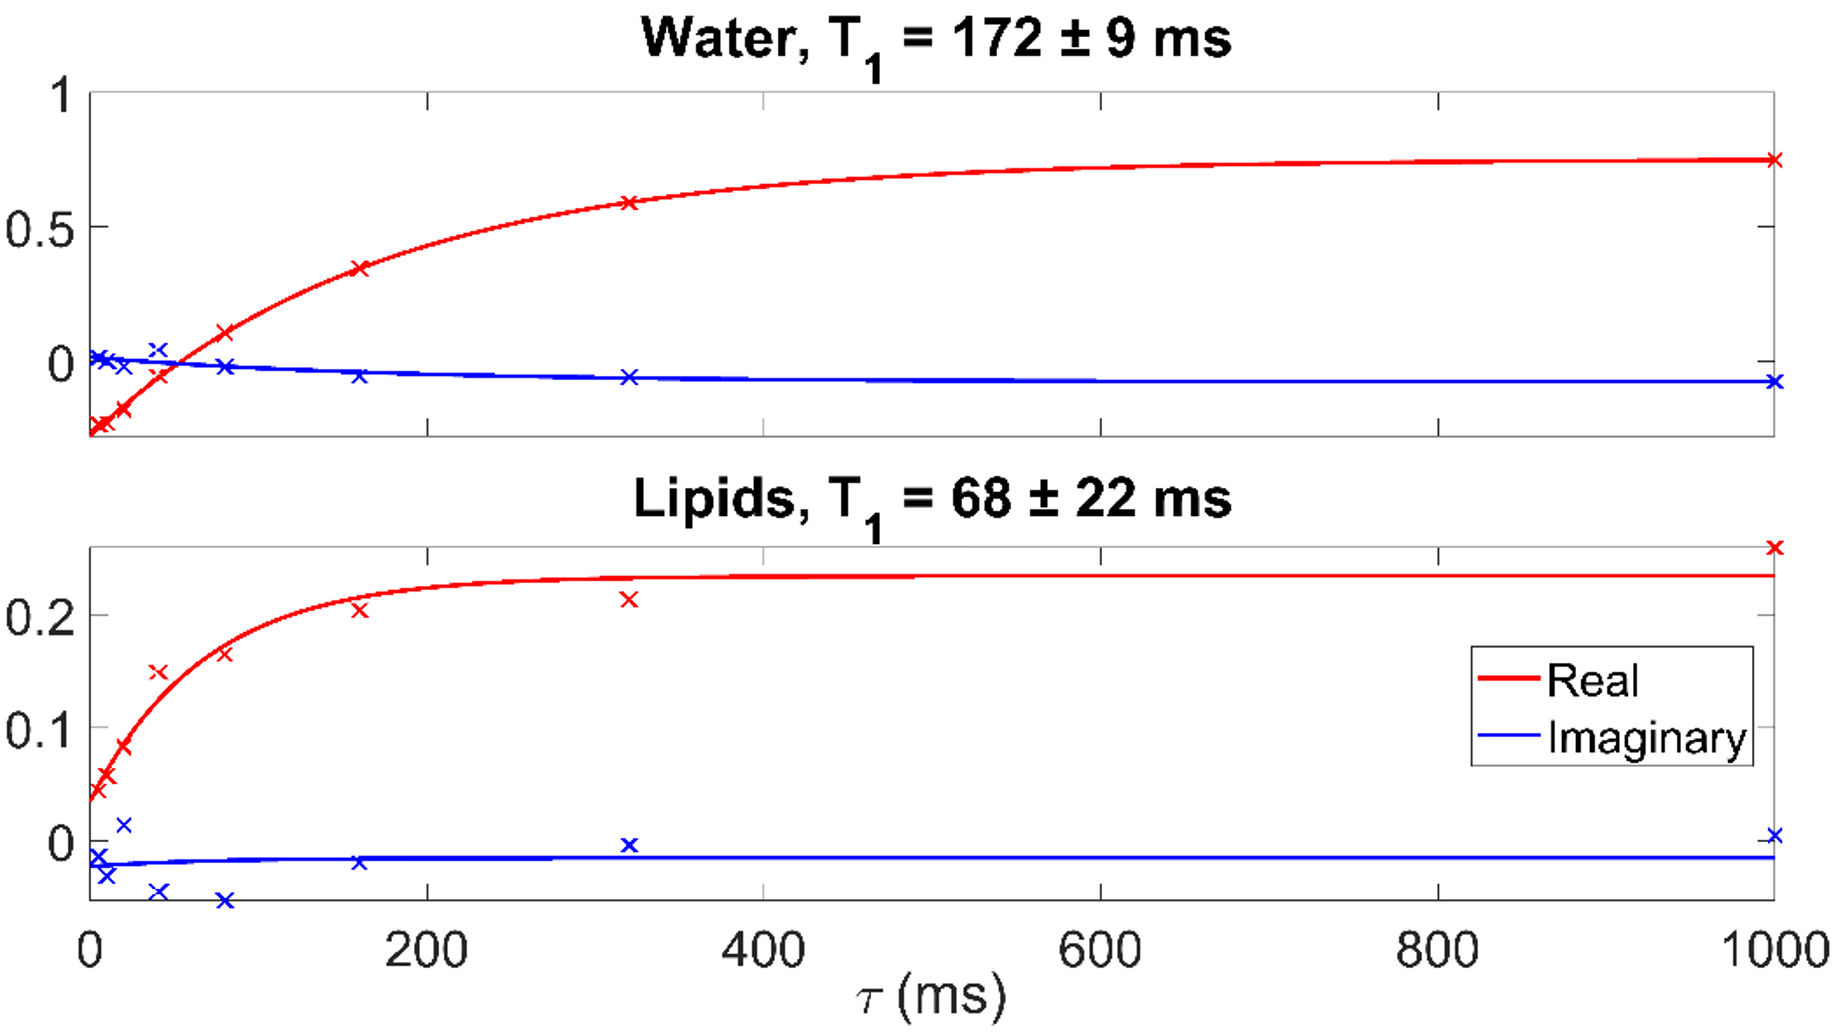
\includegraphics[width=1\textwidth]{Figures/Lipid/Amp_Tau.png}
    \caption{\textit{An example of the complex amplitudes and the fitted curves for water and lipids. Magnitude data and curves were derived (not fitted) from the real and imaginary data and fitted curves.}}
    \label{fig:Lip:Amp_Tau}
\end{figure}

\begin{table}
    \centering
    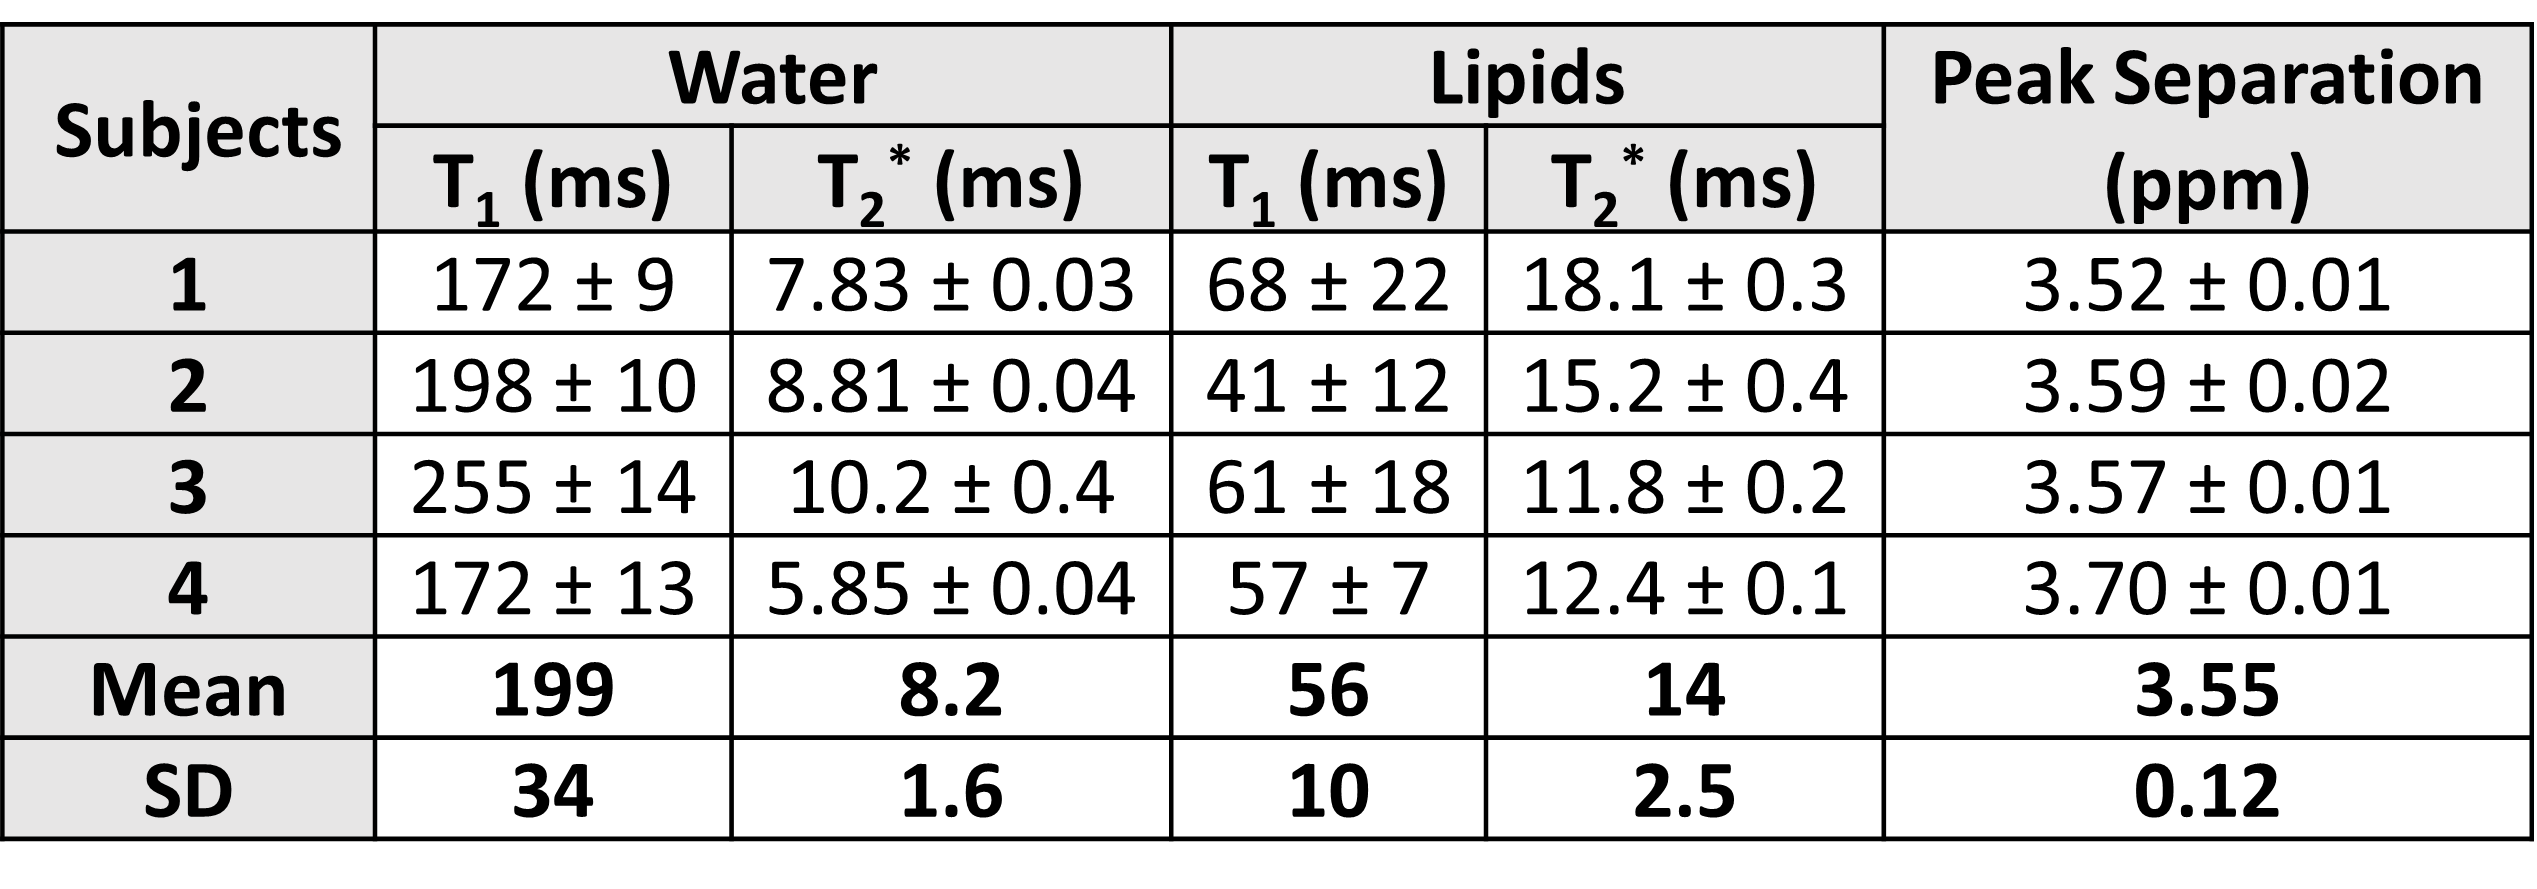
\includegraphics[width=0.9\textwidth]{Figures/Lipid/Relaxation_Table.png}
    \caption{\textit{Relaxation times of \ac{HDO} and lipids, and their chemical shift separation. Errors on values are the standard deviations obtained from the covariance matrix of the fitting. SD is the sample standard deviation.}}
    \label{fig:Lip:R_Table}
\end{table}

\subsection{Fat Increases}

\begin{figure}
    \centering
    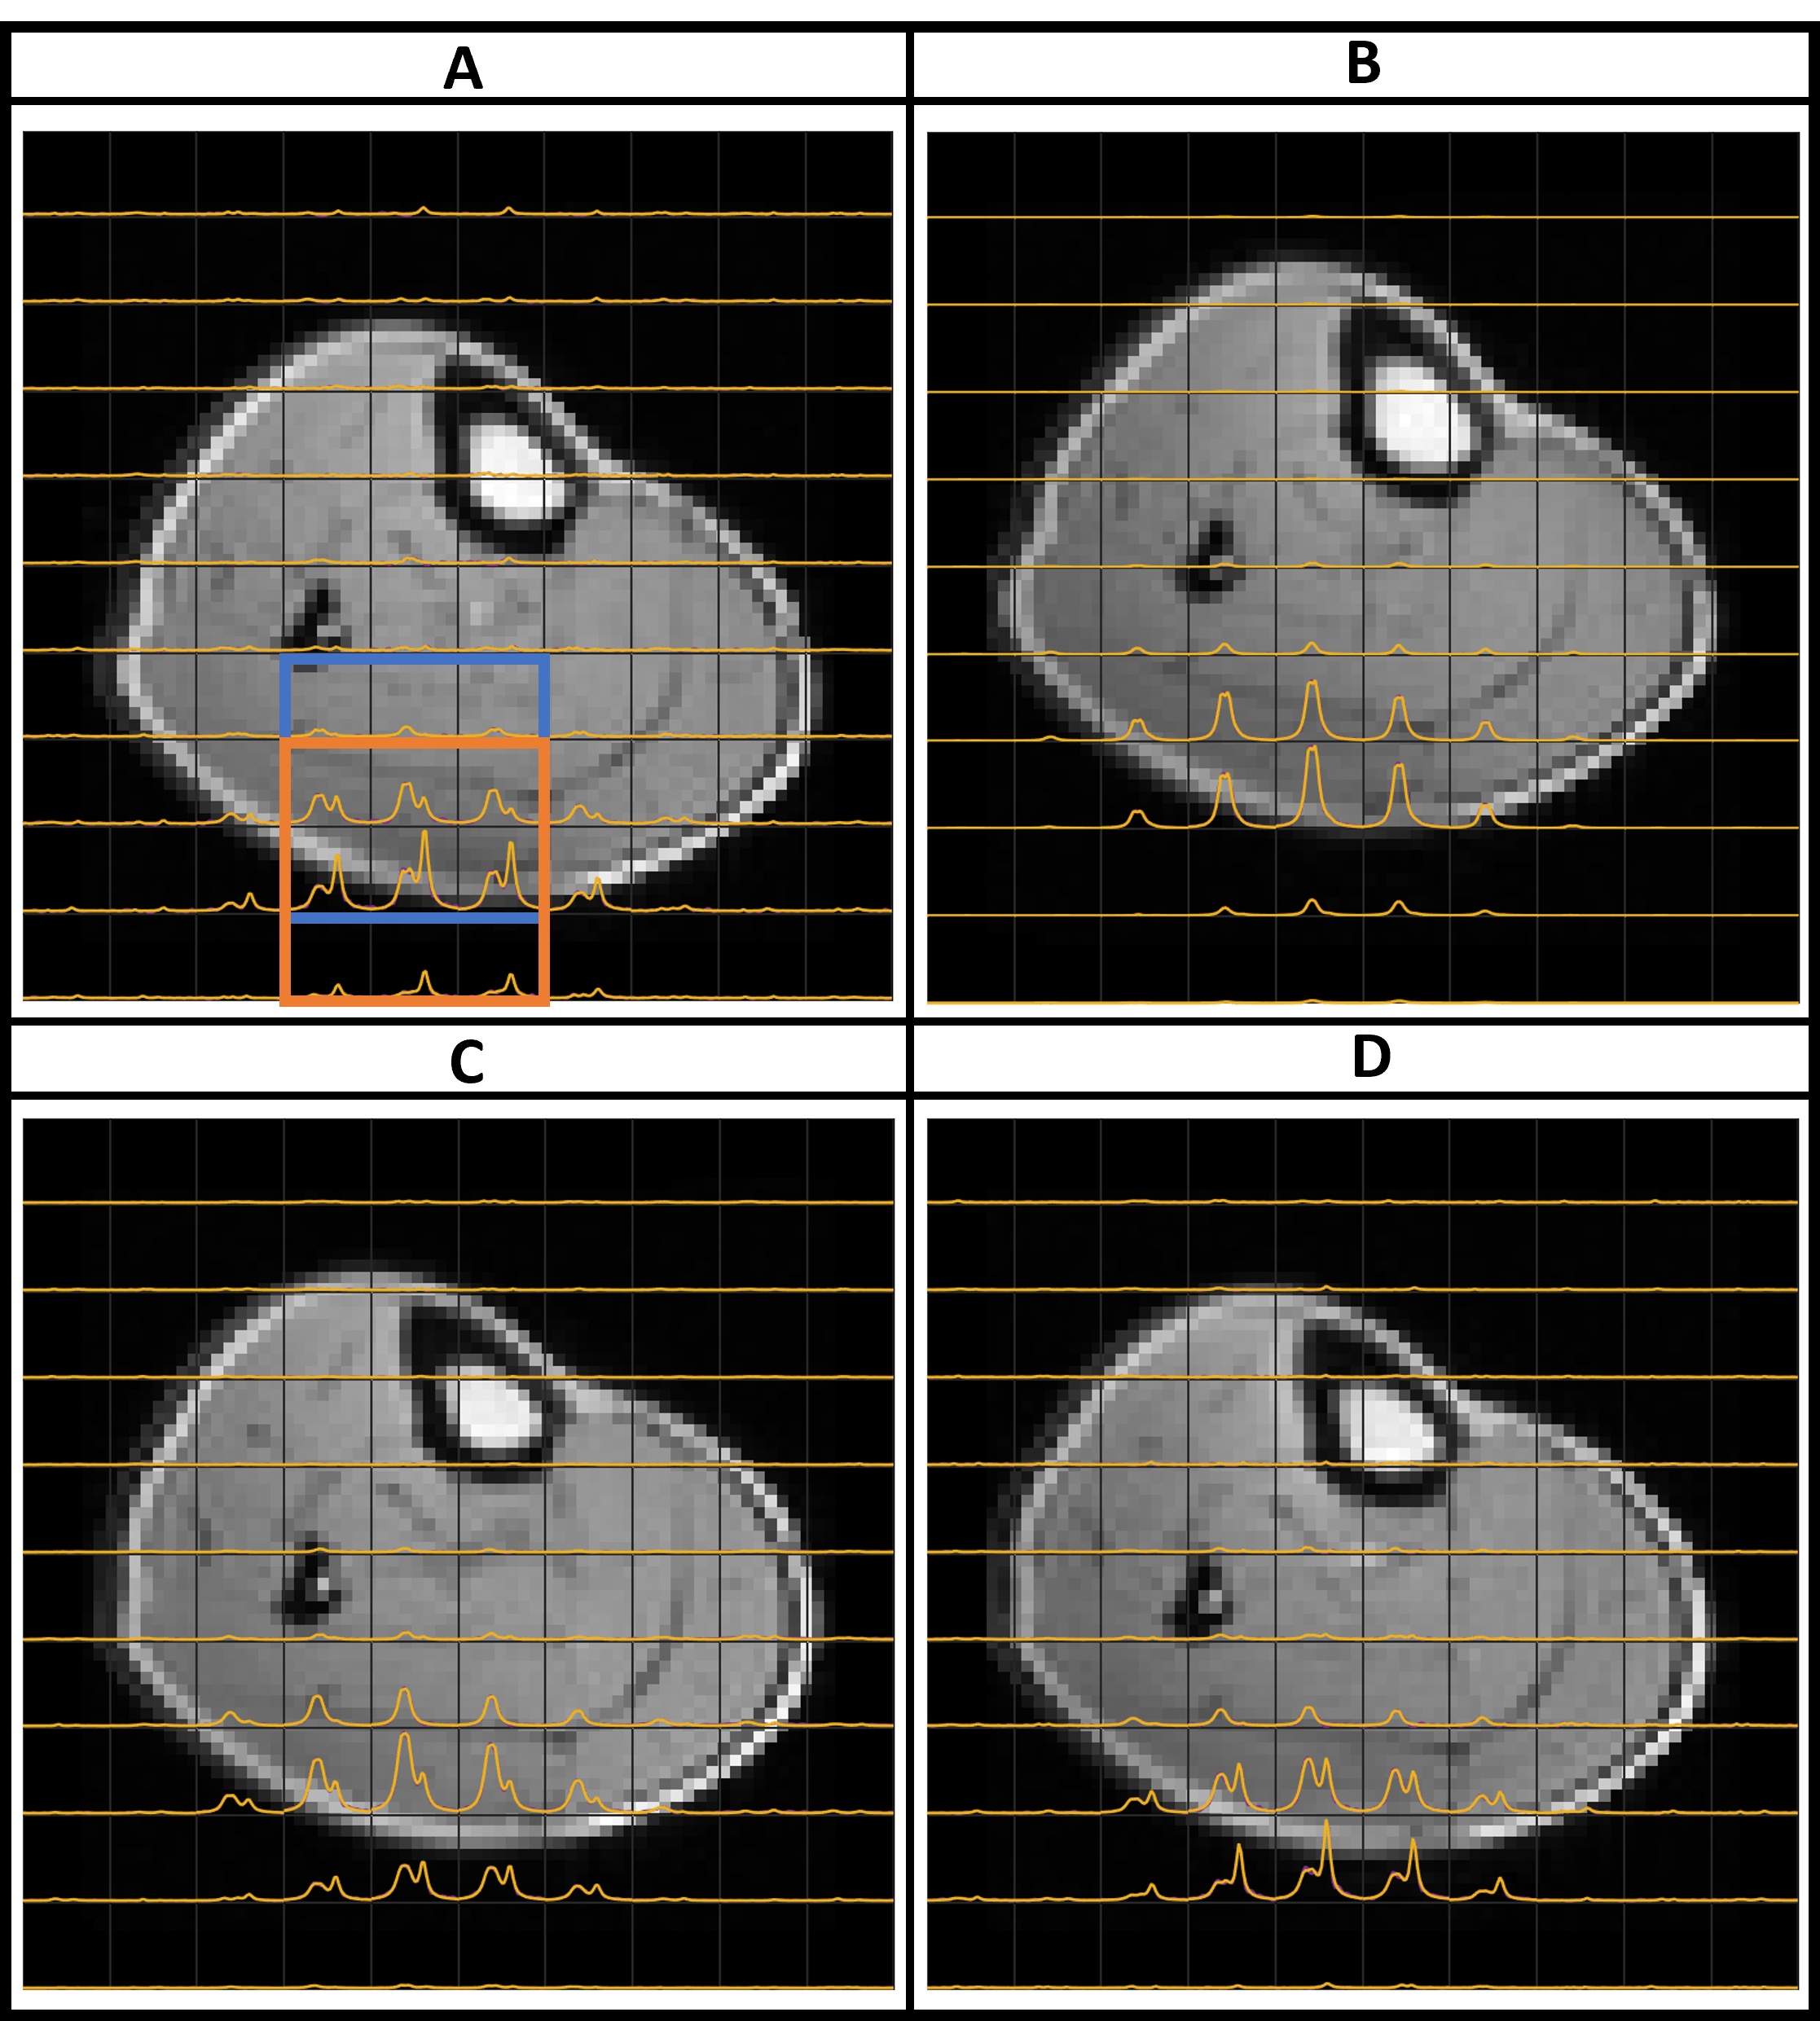
\includegraphics[width=0.9\textwidth]{Figures/Lipid/Calf.png}
    \caption{\textit{3D \ac{CSI} spectra in a single axial slice in the calf plus OXSA-AMARES fits, overlaid on corresponding $^1$H \ac{GE} images. Data was acquired from Subject 1 at four time-points: (A) at \ac{NA} before loading (t=0 days); (B) at peak loading (t=20-days); (C) after loading had ceased at t=72 days; (D) at t=113 days. ROI for signal averaging for water (blue) and fat (orange), are shown in (A). The fat \ac{ROI} was displaced by one voxel towards the surface coil to maximise sensitivity to subcutaneous fat.}}
    \label{fig:Lip:Calf}
\end{figure}

Figures \ref{fig:Lip:Calf} and \ref{fig:Lip:Abdomen} show 3D-\ac{CSI}-data acquired from Subject 1 (single transverse/sagittal slice from calf/abdomen, overlaid on $^1$H GE images) at four distinct time-points. A fat peak is seen in superficial voxels spanning subcutaneous fat close to the surface coil in the \ac{NA} images (Figs. \ref{fig:Lip:Calf} and \ref{fig:Lip:Abdomen}A), along with a water peak, which appears over a wider spatial extent and is broadened by quadrupolar splitting in calf muscle (Fig. \ref{fig:Lip:Calf}). 

\begin{figure}
    \centering
    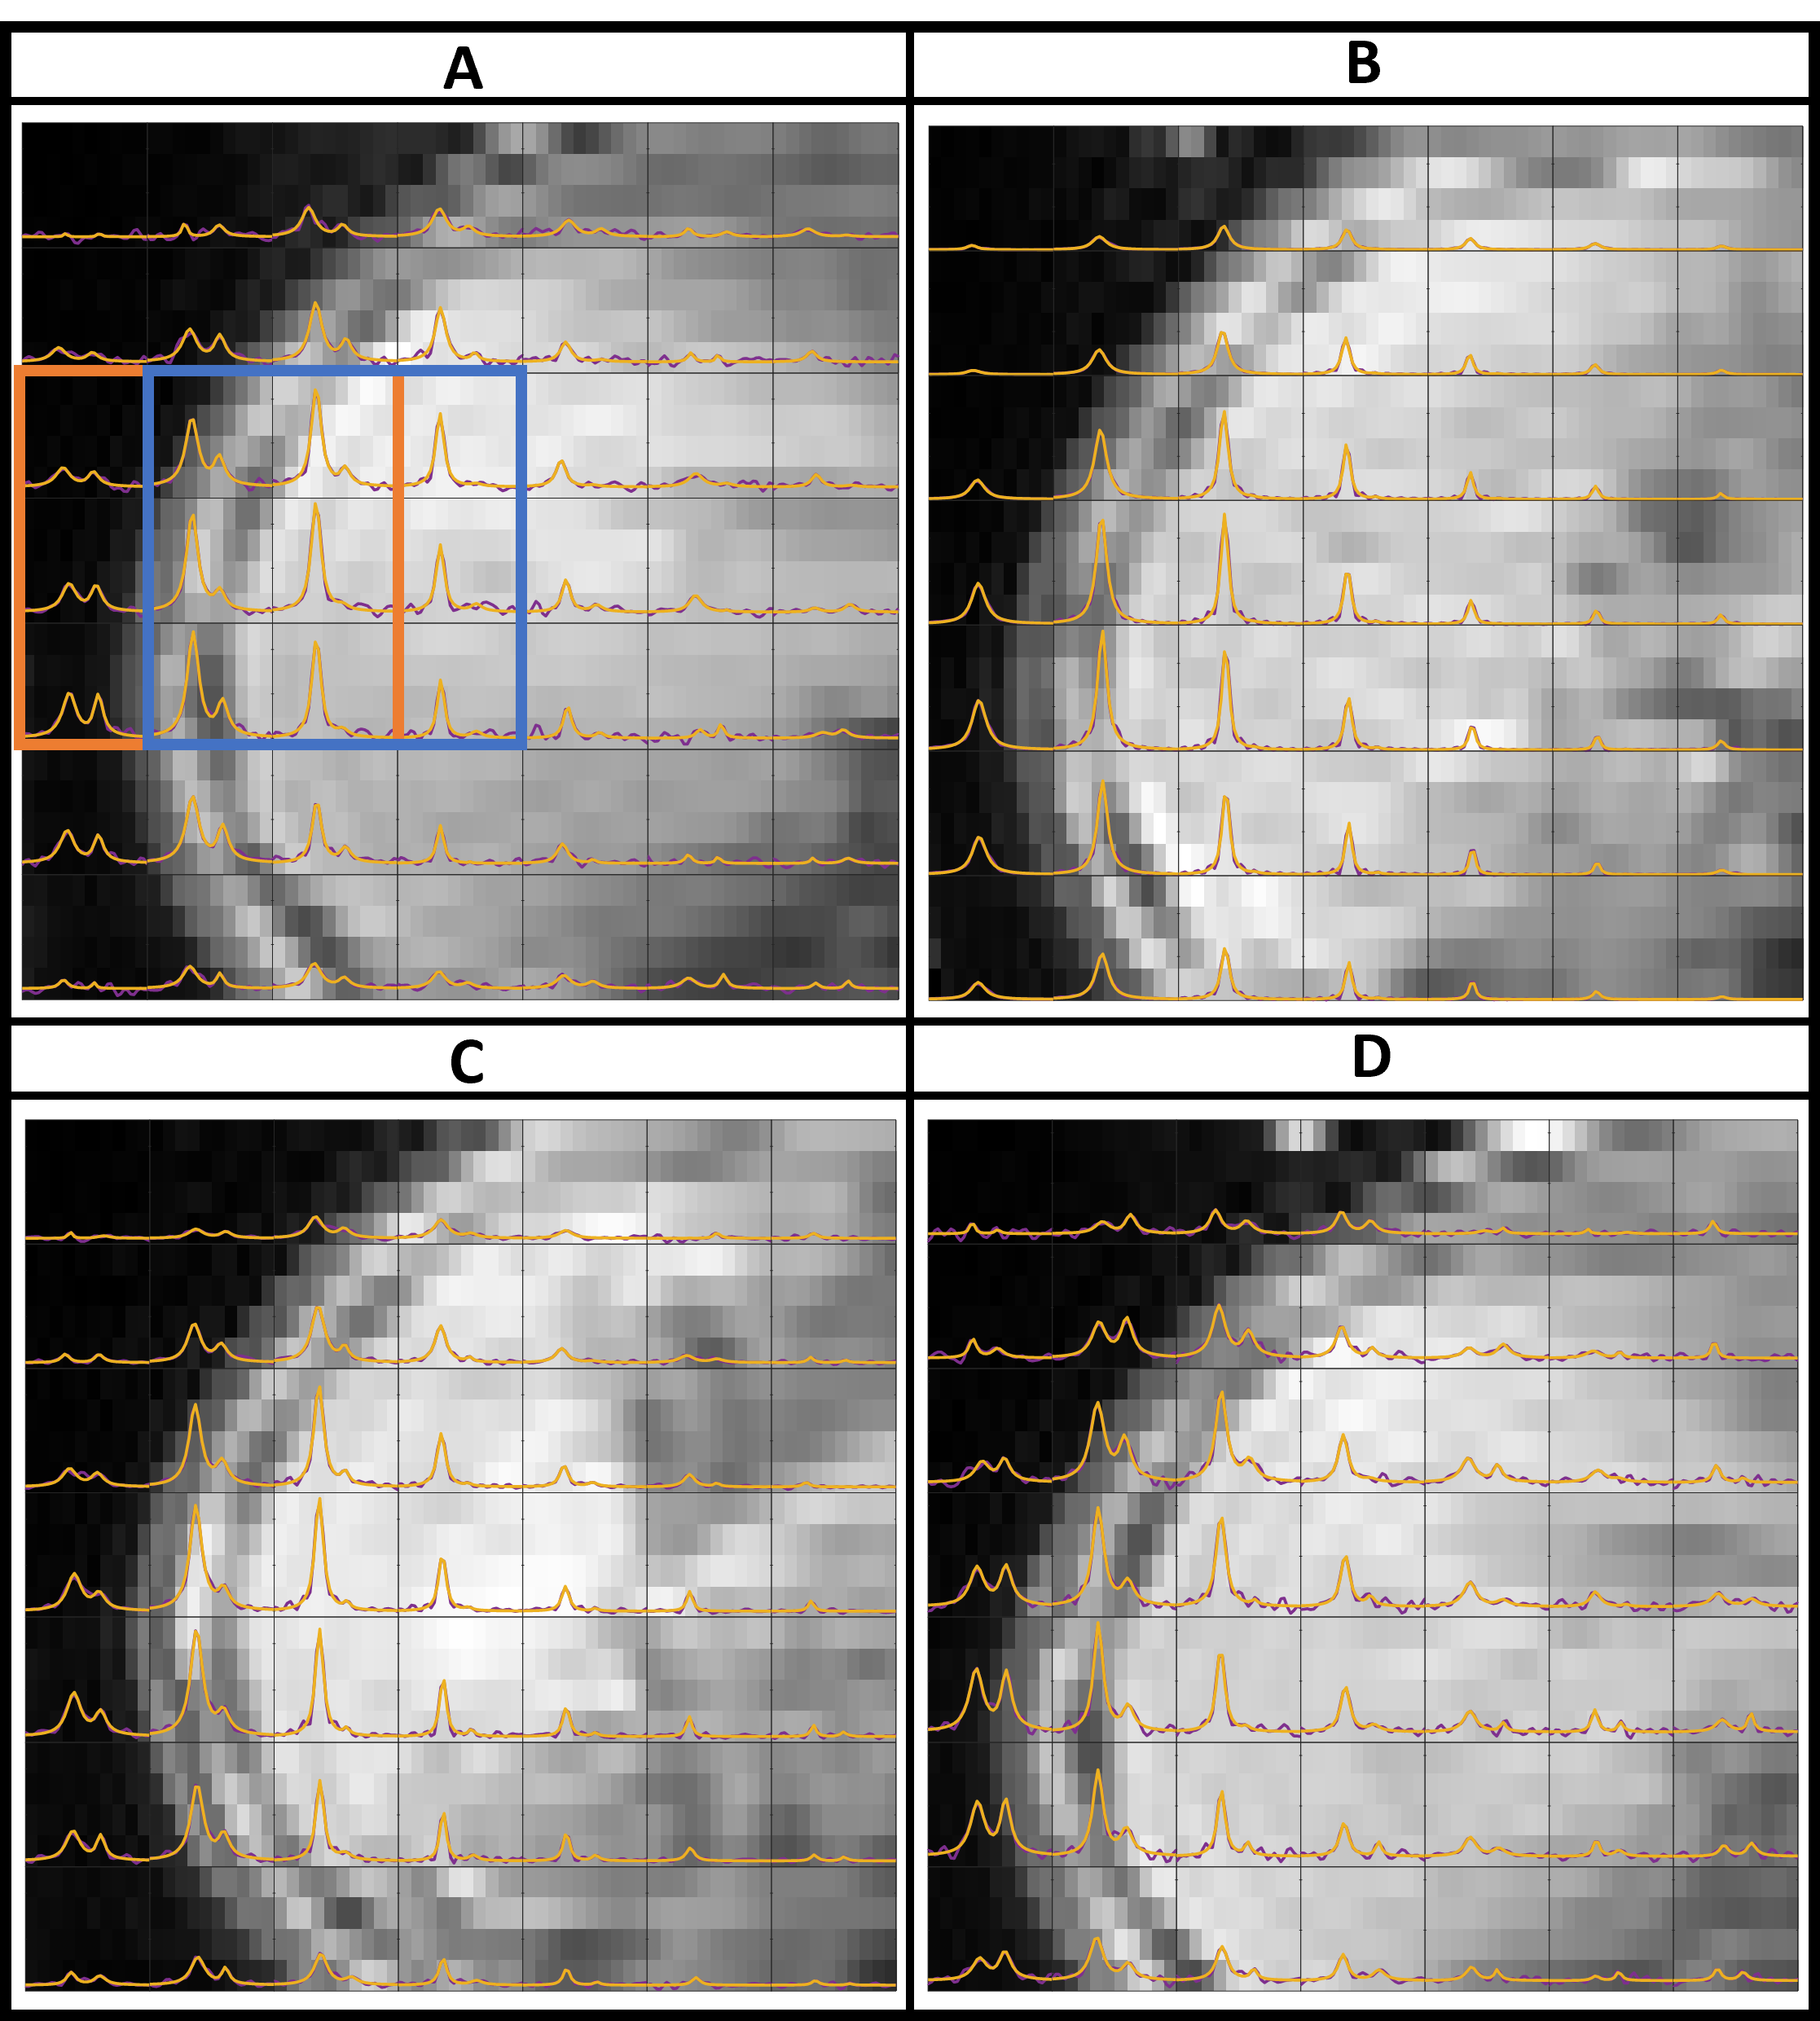
\includegraphics[width=0.9\textwidth]{Figures/Lipid/Abdomen.png}
    \caption{\textit{3D \ac{CSI} spectra in a single sagittal slice in the abdomen plus OXSA-AMARES fits, overlaid on corresponding $^1$H \ac{GE} images. Data was acquired from Subject 1 at four time-points: (A) at NA before loading (t=0 days); (B) at peak loading (t=20-days); (C) after loading had ceased at t=72 days; (D) at t=123 days. \ac{ROI} for signal averaging for water (blue) and fat (orange), are shown in (A). The fat \ac{ROI} was displaced by one voxel towards the surface coil to maximise sensitivity to subcutaneous fat.}}
    \label{fig:Lip:Abdomen}
\end{figure}

Superficial fat signals are also evident post-loading (Figs. \ref{fig:Lip:Calf} and \ref{fig:Lip:Abdomen}C,D), but during loading are swamped by the $\approx$100x larger water signal (Figs. \ref{fig:Lip:Calf} and \ref{fig:Lip:Abdomen}B) making them indistinguishable in appearance and in fitting. A robust and reliable fit to the fat signal could only be achieved at times $>$50 days when the water signal was $<$10x\ac{NA} (indicated by significantly elevated Cramer-Rao lower bound values at t$<$50 days).

\begin{figure}
    \centering
    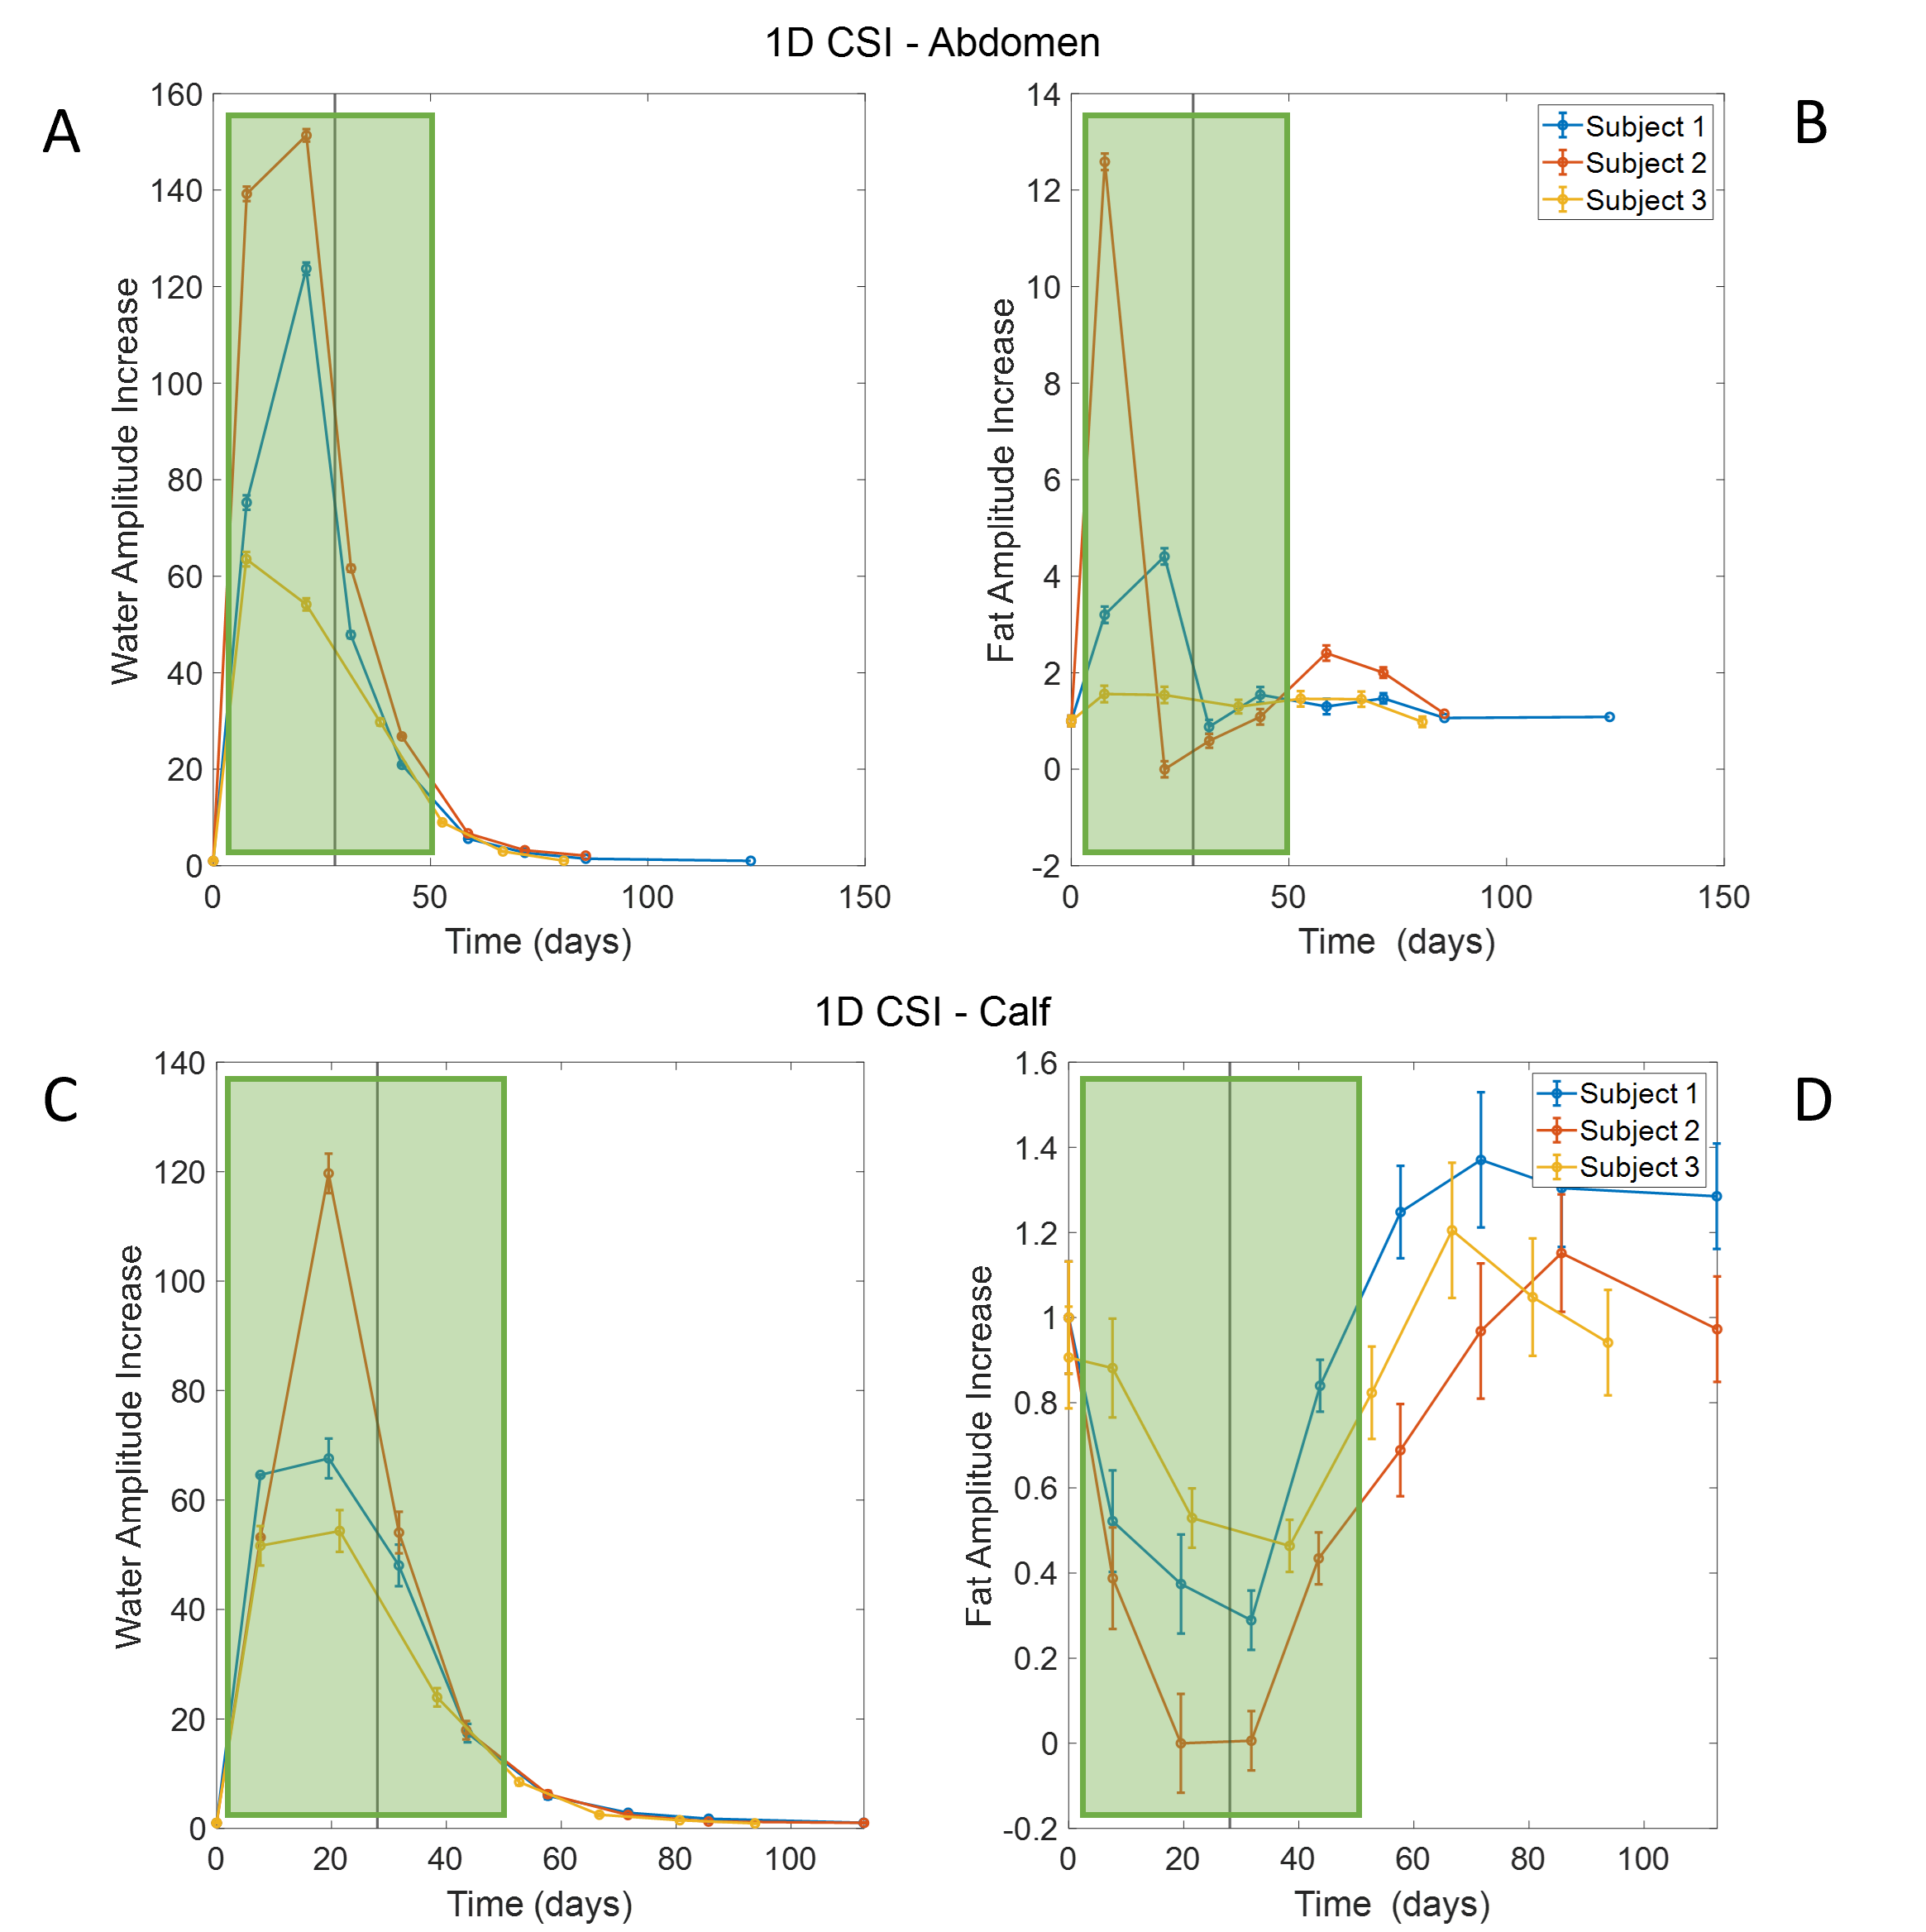
\includegraphics[width=1\textwidth]{Figures/Lipid/1DCSI_Amplitude.png}
    \caption{\textit{Plots of the temporal variation of the \ac{ROI}-averaged 1D \ac{CSI} water and fat signal amplitudes scaled by the measurement at NA for the three subjects. (A) water in calf; (B) fat in calf; (C) water in abdomen; (D) fat in abdomen. The vertical black line indicates the end of the 28-day loading period. Fat signals are only well characterised by the fitting at t> 50 days when the water signal is $<$ 10x\ac{NA}.  Error bars derived from the relative error measured from repeated experiments at NA.}}
    \label{fig:Lip:1DCSI}
\end{figure}

\begin{figure}
    \centering
    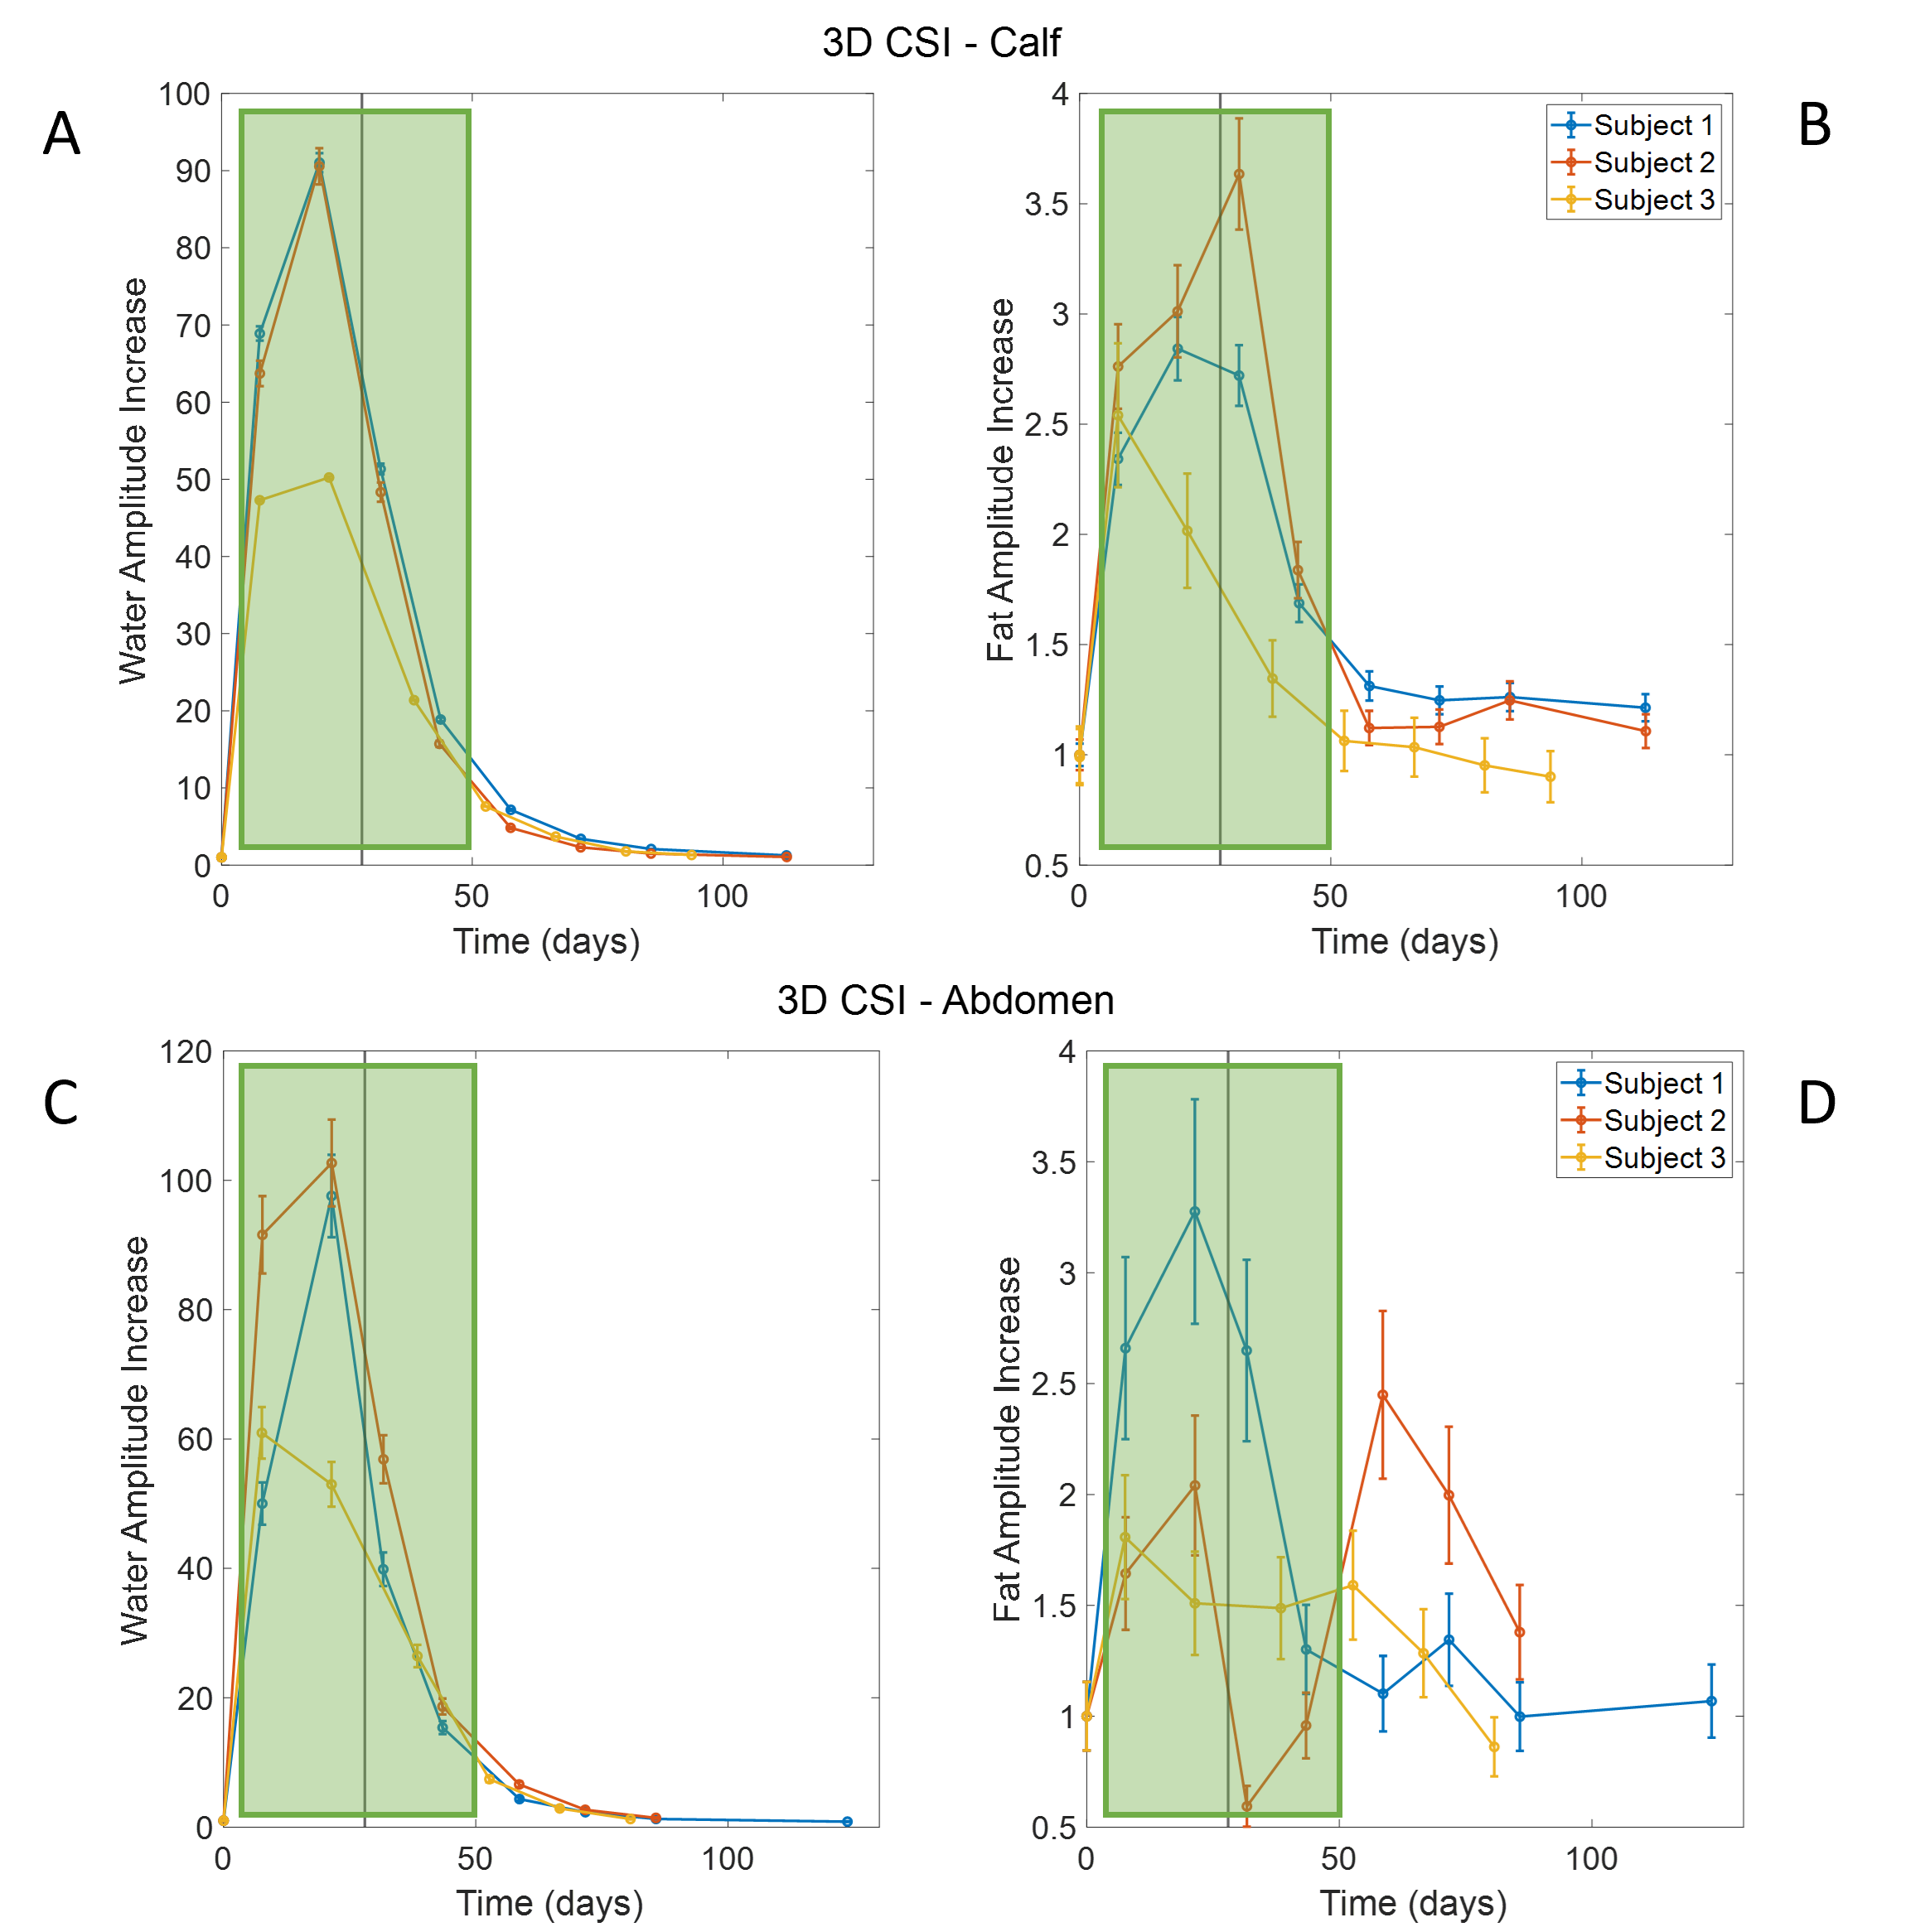
\includegraphics[width=1\textwidth]{Figures/Lipid/3DCSI_Amplitude.png}
    \caption{\textit{Plots of the temporal variation of the \ac{ROI}-averaged 3D \ac{CSI} water and fat signal amplitudes scaled by the measurement at \ac{NA} for the three subjects. (A) water in calf; (B) fat in calf; (C) water in abdomen; (D) fat in abdomen. The vertical black line indicates the end of the 28-day loading period. Fat signals are only well characterised by the fitting at t> 50 days when the water signal is $<$ 10x\ac{NA}.  Error bars derived from the relative error measured from repeated experiments at NA.}}
    \label{fig:Lip:3DCSI}
\end{figure}

Figures \ref{fig:Lip:1DCSI} and \ref{fig:Lip:3DCSI} show the temporal variation of the \ac{ROI}-averaged fat and water signals. As predicted from simulations (Fig. \ref{fig:Lip:Load}B) an increase in water signal to nearly x100 \ac{NA} is evident, with a lower enhancement in Subject 3 who loaded less (Fig. \ref{fig:Lip:Load}A). Although the fat signal shows significant early enhancement (t $<$ 50 days) this tracks the water enhancement and is likely due to poor spectral fitting. Based on the predicted long-term elevation of fat signal (Fig. \ref{fig:Lip:Load}C), we focused on the average fat signal enhancement at times $>$ 50 days where fitting was robust (Fig. \ref{fig:Lip:Amp_Table}). 

\begin{figure}
    \centering
    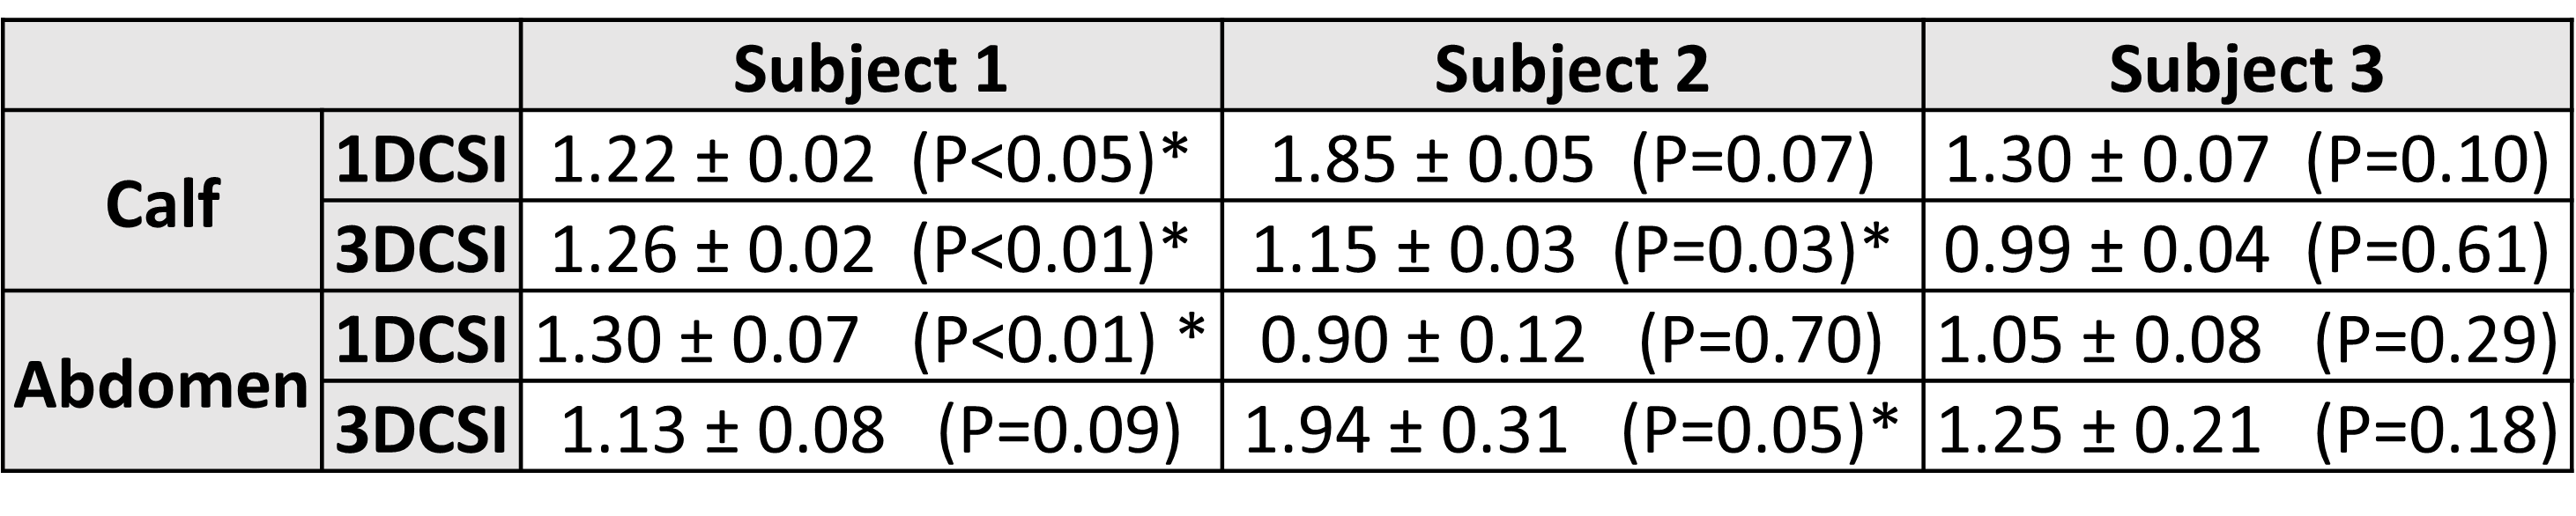
\includegraphics[width=1\textwidth]{Figures/Lipid/Lipid_Table.png}
    \caption{\textit{Average and standard errors of the fat signal enhancement relative to \ac{NA} at times of more than 50 days after the start of loading. Values are show for calf and abdomen for the three subjects. P-values for single-sided t-test for difference from \ac{NA} are also reported.}}
    \label{fig:Lip:Amp_Table}
\end{figure}

\section{Discussion}

\subsection{Comparing other Relaxation Times}

From our measurements of the lipid signal’s 3.55 ppm chemical shift, it most likely originates predominantly from deuterium in methylene groups (-CH$_2$-) of fatty acids and triglycerides, consistent with signals observed in proton \ac{MRS} \cite{Ren2008CompositionTesla}, in agreement with most previous \textit{in vivo} $^2$H measurements. In studies that administered D$_2$O to normal, obese, and diabetic mice, water and a second peak—assumed to be CHD groups from adipose tissues—were observed \cite{Brereton1986PreliminarySpectroscopy, Brereton1989TheMice}, and the position of the CHD peak was in the approximate range 3.4 $\pm$ 0.4 ppm below the water resonance. Similarly, experiments on rats produced a lipid signal at approximately 3.4 ppm below the water peak \cite{Kosenkov2018TheMice}. In contrast, during experiments on the hind limbs of mice with tumour xenografts \cite{Assmann2020InCholesterol}, an \ac{HDO} peak was observed along with a second peak at 2.8 ppm below the water position. In this case, it was suggested \cite{Assmann2020InCholesterol} that this peak arose from cholesterol (or esters of), which is actively synthesised in many tumour cells.

Previous deuterium T$_1$ measurements in muscle water produced values of 130 $\pm$ 7 ms (mouse, 9.2 MHz, 25$^\circ$C)8 and 160 $\pm$ 2.4 ms (rat, 13.7 MHz, \textit{ex vivo}) \cite{Block1987COMMUNICATIONSTissues}. Our measured values are higher, possibly due to the higher field strength and \textit{in vivo} temperature. A previous measurement of the "CHD group" found T$_1$ = 34 $\pm$ 4 ms (mouse abdomen, 30.7 MHz, in vivo) \cite{Brereton1986PreliminarySpectroscopy}, which is smaller than the value measured here. Our longer value could be a consequence of reduced accuracy caused by incomplete inversion of the lipid magnetization because of its short relaxation time \cite{Pfaff2017PredictingPulses}.

\subsection{Fat Changes}

The T$_1$ times of \ac{HDO} \textit{in vivo} that have been measured by us are larger than those measured previously in mice \cite{Fung1979StudyWater} (9.2 MHz) and rats \cite{Block1987COMMUNICATIONSTissues} (13.7 MHz). This is potentially due to the larger field strength used here. However, the fat/lipid T$_1$ that has been previously measured \textit{in vivo} in mice (30.7 MHz) is at a larger field strength and gave a smaller T$_1$ 34 $\pm$ 4 ms \cite{Brereton1986PreliminarySpectroscopy}, this could be due to reduced accuracy because of a full inversion not being achieved for lipids. 

Previous research in animal models indicates that increases in fat are still observable $\approx$20 days after loading cessation, although substantial changes in the fat signal occur prior to this point \cite{Brereton1986PreliminarySpectroscopy}. Therefore, during our measuring period of $>$ 50 days fat signal should still be increased. Fat signal was increased relative to \ac{NA} in 5 of the 6 measurements and the increase reached statistical significance (P$<$0.05) in three measurements (Fig. \ref{fig:Lip:Amp_Table}). These results provide encouraging evidence that $^2$H MR can be used to detect the increased deuteration of subcutaneous fat resulting from lipid turn-over during long-term heavy water loading. 

The wider linewidth of the \ac{HDO} signal in the calf compared to the liver is due to quadrupolar splitting induced by anisotropic muscle ordering \cite{Gursan2022ResidualMuscle}, while motion averaging in the liver mitigates this effect. This disparity makes detecting fat changes in the calf more challenging, as the lipid peak is more likely to be overshadowed by the increased \ac{HDO} signal. The main experimental challenges were in quantifying fat signals in the presence of large water signals and in reproducibility positioning the surface RF coils in repeated experiments. To optimize lipid signal detection in the calf, a smaller coil was used, which is more sensitive to subcutaneous fat, while a 12 cm liver coil was employed to measure visceral fat (though no visceral fat signal was detected). 

\subsection{Potential Improvements}

Previous research has demonstrated the feasibility of using inversion recovery sequences to nullify the HDO signal which leads to more reliable measures of changes in the fat signal \cite{Brereton1989TheMice}, especially when a dominant \ac{HDO} signal is still present. If the \ac{HDO} peak was nullified well enough consistently, spectroscopy would not be needed and imaging sequences such as \ac{FLAIR} at $^2$H resonance could be implemented. This could potentially result in higher \ac{SNR} or higher resolution. This can also be achieved post-processing through a similar technique that has been used to de-noise \ac{MRSI} data, Hankel Lanczos singular value decomposition. This technique is similar to \ac{HOSVD} except now the single values that contribute the most are removed which reduces SNR however, it can remove over-lapping water peaks and has been commonly used in $^1$H spectroscopy \cite{Jansen20061HMetabolites, Cabanes2001OptimizationBrain}.

In future work higher field could be used to provide better spectral separation of fat and water signals and 3D-printed, individualised coil holders would allow more reproducible coil positioning. This study utilized lower levels of $^2$H loading compared to previous research (2\% abundance of $^2$H compared to 10\%). Studies focused on body composition employ a similar level of heavy water loading to what was used in this study. By making these improvements it could be possible to detect visceral lipids as well as obtain earlier time-points which would mean functional/kinetic modelling could be employed to distinguish different cohorts of participants. Cohorts could include insulin resistant individuals \cite{White2017AssociationHumans} and between races \cite{White2018RacialHumans} which have already been investigated using the invasive \ac{D$_2$O} loading methodology. These studies would allow comparisons to be made for using \textit{in vivo} \ac{MRI}/\ac{MRS} methodology vs invasive biopsy methodology and hopefully therefore provide this new methodology with efficacy.

\section{Conclusion}

Water (\ac{HDO}) and lipids (probably triglycerides) were identified in the \textit{in vivo} spectra from the human calf. Relaxation times T$_1$ and T$_2^*$ were also measured and were consistent with literature values. Despite poor signal-to-noise ratio at \ac{NA} and the use of a surface coil for transceive, it was shown that such measurements are possible in a reasonable time period (approximately 30 minutes), suggesting that tracer-based metabolic studies of, e.g., triglyceride synthesis and turnover are possible in humans, and in such experimental conditions.  

The next study marks the first instance of heavy water loading being employed to track lipid signals in human participants \textit{in vivo} using \ac{MRI}/\ac{MRS} as well as without the need for biopsy. While it has been demonstrated that measuring and fitting fat peaks following \ac{D$_2$O} loading in humans is possible, further refinement of \ac{HDO} signal suppression would enhance accuracy in tracking these signals. Refinement could include higher field strength, improved coil positioning and implementation of water suppression. 

% \printbibliography % Comment out main doc

% \end{document}